\documentclass[12pt]{article}
\usepackage{fullpage}
\usepackage{graphicx, rotating, booktabs} 
\usepackage{times} 
\usepackage{fbb} 
\usepackage{natbib} 
\usepackage{indentfirst} 
\usepackage{setspace}
\usepackage{grffile} 
\usepackage{hyperref}
\usepackage{tikz-cd}
 \usetikzlibrary{cd}
\usepackage[export]{adjustbox}
\usepackage[most]{tcolorbox}
\usepackage{verbatimbox}
\usepackage{lscape}
\usepackage{afterpage}
\usepackage{amsmath}
\usepackage[labelfont={bf},textfont=it,labelsep=period]{caption}
 \usepackage{multirow} 
\setcitestyle{aysep{}}
\usepackage{dcolumn}

\hypersetup{
  colorlinks = true,
  urlcolor = blue,
  linkcolor = black,
  citecolor = black,
  pdfauthor = {Joshua Alley},
  pdfkeywords = {},
  pdftitle = {},
  pdfsubject = {},
  pdfpagemode = UseNone,
%  pdffitwindow = true
%  pdfcenterwindow = true
}



\singlespace
\title{\textbf{Arms and Elections: Arms Deals with Autocracies, Defense Contracting and U.S. Presidential Elections}}
\author{Joshua Alley \\
Assistant Professor \\
University College Dublin\thanks{Thanks to Brian Blankenship, Rosella Capella, Jonathan Caverley, Jonathan Chu, Ben Fordham, Erik Lin-Greenberg, Zachary Markovitch, Leah Matchett, Andy Philips and Phil Potter, as well as participants in the Boston University Political Economy of Security Online Workshop Series and 2022 Meeting of the International Studies Association for helpful comments.} \\
joshua.alley@ucd.ie \\
\\
Word Count: 9,796
}

 
\date{\today}

\bibliographystyle{apsr}

\usepackage{sectsty}
\sectionfont{\Large}
\subsectionfont{\noindent\large\textit}
\subsubsectionfont{\normalsize}

\makeatletter
\renewcommand\tiny{\@setfontsize\tiny{9}{10}}
\makeatother


\begin{document}

\maketitle 

\begin{abstract} 
The United States makes more arms deals with autocracies during election years. 
U.S. leaders sell arms to autocrats to bolster their electoral prospects by claiming credit for providing jobs and increasing defense contracting.
Autocratic arms recipients have the political flexibility to order arms around elections and increase their security by taking arms. 
I provide three pieces of evidence for this argument.  
First, I detail electoral cycles in arms deals between the United States and autocracies. 
I then show that arms deals increase defense contract awards in swing states.
Finally, I unpack the process by showing how deal timing shifts after regime change, that U.S. allies drive most of the autocratic arms deals cycle and that the same platforms that move in arms deals increase swing state contracts.  
The argument and results detail the electoral motivations of U.S. security cooperation with autocrats. 
\end{abstract} 



\newpage 
\doublespace 


\section{Introduction}



% US-Brazil 1972
In 1972, the Nixon administration finalized ten deals to transfer or sell arms to Brazil.
Over the next four years, Brazil's military junta received 500 M-113 armoured personnel carriers, five destroyers, seven submarines, and eight S-2E Tracker anti-submarine warfare aircraft.
These deals came while Nixon sought reelection and arms deliveries continued after his 1974 resignation. 


% Obama 2012
Something similar happened during the 2012 presidential election, when Saudi Arabia ordered arms from the Obama administration.\footnote{Obama first announced the deal in 2010. I analyze confirmed orders, not announcements.} 
Twelve deals included 400 Harpoon anti-ship missiles, 12 Apache attack helicopters, and 63 K-6 120mm mortars, along with F-15 jet parts, guided bombs, and other helicopters \citep{SIPRI2021}. 
The resulting deliveries spanned the next eight years, and supported the 2015 Saudi intervention in Yemen's civil war.


% puzzle/question 
Substantial arms sales to autocracies often coincide with U.S. presidential elections because domestic political competition in the United States encourages arms deals with autocracies. 
Around elections, U.S. leaders make more arms deals with autocracies in order to claim credit for defense industrial jobs and increase defense contracting.
New defense contract awards then flow to swing states, improving or maintaining economic conditions in critical electoral regions.
Arms deals with autocracies thus bolster leaders' efforts to retain power via political budget cycles \citep{Tufte1978, Mintz1988, DerouenHeo2000}. 


% example- PBC consequences vary w/ security coop
% arms exports logic
Autocracies buy arms near U.S. elections because arms transfers increase their security and autocrats have additional political flexibility. 
Unlike democratic leaders, who face institutionalized budget processes and opposition scrutiny, autocrats have fewer constraints on accommodating electoral cycles.
Buying arms then fortifies autocracies against external and internal threats.
Buying arms is particularly important because arms sales are central to security cooperation between the United States and autocracies \citep{Yarhi-Miloetal2016, McManusYarhi-Milo2017}.
%These arms export cycles reinforce cooperative relationships between U.S. leaders and alliance prot{\'e}g{\'e}s. 



% Findings
I provide three pieces of evidence to support this argument.
First, I find that U.S. arms deals with autocracies increase during election years, especially presidential elections, while arms deals with democracies are unchanged. 
Second, I show that arms deals have little association with contracts outside of swing states, but increase contract awards in swing states. 
Finally, I corroborate these correlations by examining the process in three ways.
The first check addresses autocratic constraint by comparing deals before and after democratization in Greece and Portugal. 
After that, I document the importance of autocratic security motivations by showing that autocratic allies who rely on the United States for security drive election-year arms deals. 
Last, I examine which weapons systems move in deals and increase swing state contracts, and find that aircraft, ships and vehicles all contribute to deals and contracts, and aircraft have the largest role. 


% focus on the U.S.
%The pivotal economic and security roles of the United States make understanding the economic and security consequences of U.S. electoral competition worthwhile. 
%The United States is the leading arms exporter, maintains expansive alliance ties, and there is prior evidence that leaders use defense contracting for electoral advantage \citep{DerouenHeo2000}. 
%Other states might leverage security cooperation to facilitate different policy cycles, however. 


% economic and seucrity ties 
The argument and findings address three salient issues in international relations. 
First, this paper details the electoral causes of security cooperation. 
Just as domestic political business cycles in large countries reshape economic conditions \citep{Kayser2006}, electoral competition alters U.S. security cooperation. 
%That security cooperation then reshapes U.S. politics in turn. 


Specifically, electoral considerations provide a new explanation of when, why and to whom the United States sells arms. 
Existing work on arms transfers considers diverse reasons why states make arms transfers \citep{WillardsonJohnson2022}, including foreign policy interests \citep{Thralletal2020}, economic considerations \citep{Bitzinger1994} networks \citep{Thurneretal2019}, and leverage \citep{Spindel2023}. 
Using arms sales for electoral advantage adds to these findings, and is particularly important because the United States is the leading arms exporter.


Last, my argument and findings help clarify why the United States often sells arms to autocracies despite normative and geopolitical concerns. 
While strategic interests and other common determinants of arms exports create a baseline flow of arms between the United States and some autocracies, electoral competition adds further motivation. 
Autocracies have sufficient political flexibility to make arms deals near elections and reap security benefits by doing so. 


% this is a cut candidate
%Last, my results mirror prior findings that antagonistic foreign states can use economic policies to impact electoral competition. 
%For instance, China used tariffs to reduce Republican vote share in the 2018 midterm elections by targeting industries in competitive districts, and soy tariffs to hurt Republican congressional candidates in soy-producing areas \citet{ChyzhUrbatsch2021, KimMargalit2021}. 
%My argument considers how security partnerships can help leaders manipulate economic conditions to their advantage. 


% need an outline 
This paper begins by outlining the potential instruments of political business cycles in the United States, the importance of defense contracting, and how elections encourage arms deals with autocracies. 
I then test several implications of the argument. 
First, I test how partner regimes and presidential election timing shape U.S. arms deals from 1950 to 2014.
I then show that arms deals are correlated with increased defense contract awards to swing states.
Finally, I unpack the process by analyzing arms deals before and after democratization within two NATO members, the role of autocratic security concerns and which weapons move both deal cycles and swing state contracts.
The last section discusses the results and concludes.


\section{Argument}


Electoral competition encourages U.S. leaders to make additional arms deals with autocracies.
To begin, I detail constraints on aggregate budget cycle tools and discuss why defense contracting is an attractive way to manipulate economic conditions.
I then describe how arms deals can accelerate defense contracting. 
Finally, I explain how low political constraints and security considerations make autocracies able and willing to buy arms around U.S. elections.


Elections impact policy \citep{Nordhaus1975}.
%\footnote{See \citet{Dubois2016} for a review of political budget cycle scholarship.} 
When leaders want to retain office, they attempt to improve economic conditions and win votes. 
Leaders create political budget cycles by using fiscal and monetary policy to increase economic growth near elections.
This helps hold power for themselves or their party \citep{Tufte1978, Rogoff1987}. 


In the United States, however, leaders cannot easily manipulate macroeconomic policy to improve their electoral prospects.  
Federal Reserve independence limits political influence on monetary policy \citep{ClarkHallerberg2000}. 
In fiscal policy, aggregate budgets constrain spending discretion.


Recent political cycles scholarship in therefore emphasizes targeted policies.
Focused manipulations maximize electoral impact by prioritizing key constituencies \citep[pg. 248]{Dubois2016}.
For example, U.S. leaders often initiate trade disputes for industries in swing states as elections approach \citep{Conconietal2017}.%\footnote{Elsewhere, leaders use labor agreements \citep{Ahlquist2010} and land reform \citep{Philips2020} to win support in key blocs.} 


% Defense spending/contracts as flexible instrument
Scholars have long speculated that defense spending is a useful instrument for budget cycles (e.g. \cite{Tufte1978, Mintz1988}).
Leaders have discretion in allocating military spending, and defense spending often serves social welfare goals \citep{WhittenWilliams2011}.
\citet{Becker2021} finds that unemployment encourages NATO members to shift spending from equipment to personnel, for instance.


% in US context, contracts
U.S. defense budgets are poor cyclical tools, however, as Congress makes allocations two years ahead.
Defense contracting has more flexibility, as presidents control contract timing and disbursement \citep{Mayer1995, DerouenHeo2000}.
Leaders can also focus on key constituencies and claim credit for awards \citep{DerouenHeo2000}. 
%Targeted spending generally increases support for incumbents \citep{KrinerReeves2012}, and defense contracts can be a targeted instrument.


In the United States, presidents who want to maximize the electoral impact of defense contracts will focus on swing states.
These consistently competitive states hold the balance of the Electoral College \citep{KrinerReeves2015}. 
Many swing states such as Florida and Pennsylvania also have defense firms that can benefit from contracts.
Their defense industrial base may be smaller than less electorally competitive states like California, Texas, and New York, however. 


Presidents cannot simply disburse contracts to swing states, however. 
The defense budget sets contracting levels. 
Also, if leaders want to award more contracts and expand or maintain defense production, the U.S. military may not need older systems or lack absorption capacity to incorporate new outputs.
Political increases in the supply of defense contracting may not respond to military needs, so finding other buyers is necessary.


Foreign markets provide additional demand for defense goods.
Other countries can buy new production or sustain production lines for older equipment. 
U.S. leaders can also sell or transfer old equipment to make room in U.S. stocks or award contracts for refurbishment. 
When U.S. leaders turn to foreign buyers of defense goods, using defense contracting for political gains has international spillovers.\footnote{% Political Business cyles
This is analogous to the international economic consequences of budget cycles. 
\citet{Ito1991} finds that U.S. elections increase economic growth in Japan, while \citet{FoersterSchmitz1997} argue that U.S. electoral cycles impact international stock returns.
}


% timeline and intermediate goods
Arms deals provide two electoral benefits, and leaders only need arms deals and confirmed orders to reap them.\footnote{Final transfers can and often do come years later. 
Only 23\% of deals result in deliveries in the same year, and the median lag between orders and the first delivery is one year. 
As a result, arms deals are more likely to follow electoral cycles than transfers of finished defense goods, as production times vary widely. 
Ships, tanks and planes can take years to assemble.
Munitions and smaller platforms move faster.}
First, when they announce a deal, leaders can highlight how they are creating or protecting defense industrial jobs. 
Such credit claiming is essential to budget cycles \citep{Bueno2021}. 
Second, as confirmed orders stimulate contract awards, economic conditions substantiate claims that leaders are protecting jobs. 


Other scholarship suggests that using arms deals and contracts to build electoral support works. 
Targeted spending boosts support for incumbents \citep{KrinerReeves2012}.
Bringing in funds while claiming credit also increases support for leaders \citep{Grimmeretal2012}. 


% preservation vs creation
When leaders argue that arms sales create and preserve jobs, preservation may be more important than creation. 
Arms sales add relatively few jobs, but selling older equipment sustains established production lines \citep{Caverley2018}. 
Maintaining employment avoids negative shocks in regions with fine electoral margins. 


% Credit claiming examples
U.S. leaders regularly claim that arms deals support defense industrial employment. 
The Obama administration used jobs to justify the \$60 billion sale to Saudi Arabia.
Boeing and U.S. officials highlighted 14,000 jobs tied to Saudi purchases of F-15 jets, for instance \citep{hillsaudisale2010}.
Donald Trump then attempted to claim credit for jobs tied to existing Saudi deals or letters of intent. 
In 2020, a Department of Defense press release claimed that among U.S. workers, "up to 1 million ... depend on U.S. defense exports for their job security'' \citep{dodarmsjobs2020}. 


Other Presidents used similar rationales for arms sales.
The Nixon administration advanced jobs and employment as one of several justifications for arms sales \citep[pg. 34]{Sorley1983}. 
When the Clinton administration engaged in far more arms sales than observers anticipated, jobs had an important role.
One defense industry executive argued that ``Clinton realizes these exports create jobs'' \citep{clintonarms1993}.
%Concerns that reduced defense spending at the end of the Cold war would impact employment led Clinton's commerce secretary to argue that a ``critical piece of the defense conversion puzzle is helping firms find export markets'' 


% Congress- rarely blocks sales- occastional conditions 
Highlighting the economic benefits of arms deals also helps leaders secure Congressional approval. 
While the executive branch negotiates arms sales, Congress can veto deals with a joint resolution. 
For Congressmen and Senators who themselves face re-election and may benefit directly, opposing deals is risky.
For this and other reasons, Congress has never successfully blocked an arms deal, and relies on conditions and monitoring \citep{Thralletal2020}.\footnote{Congress blocked a 2019 arms sale to Saudi Arabia, but Trump vetoed the joint resolution.}


% announcements and orders don't always line up  
Congressional approval is necessary for a foreign customer to place orders. 
As a result, there is often a gap between deal announcements and actual orders.
Leaders will therefore negotiate and announce deals so that orders arrive near elections.  


Even with delays between announcements and orders, arms sales are still a useful vehicle for increasing defense contracting. 
Executive leaders and Congressmen can and do highlight jobs when they first announce a deal. 
Moreover, leaders can expect Congressional approval, so orders ultimately provide material benefits in key electoral areas. 


% additional production and foreign markets
%When defense production and planning diverge, foreign markets provide alternative takers for excess arms production from defense contracting cycles. 
When U.S. leaders attempt to use arms deals to stimulate defense contracting, not every country is a useful partner. 
While all states could make deals, democracies face budget and political constraints and have alternative sources of security.
In contrast, autocracies have more political flexibility and rely more on U.S. arms for security.



\subsection{Arms Deals with Autocracies}


Autocracies are more likely to buy U.S. arms near elections. 
Autocrats have more political freedom to respond to U.S. leaders' growing interest in arms deals near elections, because they have fewer policy and opposition constraints than democratic leaders. 
Autocrats are also especially inclined to seek arms because arms transfers are central to U.S. security cooperation with autocracies.
As a result, autocrats buy arms near elections because they have consistent motivation to buy U.S. arms and additional opportunity to do so. 


% constraints
Autocracies have greater political flexibility to make arms deals around elections than democracies. 
Democratic leaders might face criticism of deals for U.S. arms.
Other elites could object to spending on arms, competition for domestic arms manufacturers, or excessive alignment with the United States.


% laws and budget processes
Routine budget processes also constrain democratic leaders.
Asking for additional appropriations to purchase arms is politically risky, because it invites scrutiny. 
As a result, democracies may make arms deals within existing security institutions, but will not buy arms near U.S. elections.


% less security need
In addition to political constraints, democracies have less security need to make arms deals. 
Joint democracy promotes formal alliances and deep security cooperation, which gives democracies additional security without purchasing U.S. arms. 
Peacetime military cooperation between democracies in institutions like the EU and NATO also promotes joint arms production \citep{Klare1983, Bitzinger1994}.
Joint production adds consistency to arms transfers. 
Democracies engage in joint production to secure domestic political benefits from defense jobs and cooperate with their security patron.
Democracies also benefit from other commitment signals \citep{McManusYarhi-Milo2017}. 
%High and consistent arms deals follow. 


Potential opposition criticism, budget constraints, and alternative security arrangements mean that buying U.S. arms near presidential elections is unlikely to help democratic leaders.
Democratic leaders run political risk for minimal security gain if they engage in opportunistic arms purchasing. 
As a result, democracies will still buy U.S. arms, but they will do so are part of structured, consistent cooperation with little room for increased purchases near elections. 


Autocrats have less political constraint and different security needs.
Even if other autocratic elites oppose additional outlays on U.S. arms, scrutiny of deals is less likely challenge an autocrats' power base. 
Autocracies also need not respect a codified budget process, so they have more financial flexibility.
As a result, autocrats can buy U.S. arms around elections, when U.S. leaders especially seek export markets.   


% offstage signaling and need
Buying arms helps autocrats bolster their security.
In general, states can build weapons at home, buy arms from abroad, or employ alliances to bolster their military capability. 
Autocratic security partners of the United States often rely on purchasing arms, because they have less sophisticated domestic defense industries \citep{Bitzinger2003} and weaker formal alliance ties \citep{Yarhi-Miloetal2016}. 


% explain why 
Domestic politics constrains formal alliances and other signals, so arms transfers are pivotal to U.S. security cooperation with autocracies.  
The United States prefers ``offstage'' signals of support for autocrats, rather than public demonstrations of commitment \citep{McManusYarhi-Milo2017}.
Furthermore, U.S. public opinion favors security cooperation with democracies \citep{Alley2023}. 
For autocrats, formalizing an alliance might promote democratization \citep{GiblerWolford2006}.



While arms transfers complement U.S. security commitments to democracies, sales substitute for public signals, peacetime cooperation and joint production in security guarantees to autocracies.
In some cases, arms transfers substitute entirely for formal security guarantees \citep{Yarhi-Miloetal2016}. 
Because arms are essential to U.S. security commitments, autocrats will buy arms to increase their military capabilities.
This mirrors how democracies can use aid to get foreign policy concessions from autocracies, but not democracies \citep{BDMSmith2009}.\footnote{Arms transfers may not provide much leverage, however \citep{Spindel2023}.}


% internal
Internal security concerns further motivate autocratic deal-making. 
Maintaining a robust coercive apparatus is essential to autocratic leaders' survival in office \citep{Boix2008}. 
U.S. arms can provide coercive capacity or allow leaders to invest in repressive capabilities by substituting for other defense goods. 


Arms deals around elections further increase autocracies' security by currying favor with U.S. leaders.
Autocrats can certainly understand the electoral incentives of U.S. leaders and leverage their political flexibility to buy more arms at helpful times. 
This cooperative behavior and support for U.S. defense industrial jobs is likely to increase U.S. elite support for continued security cooperation, which bolsters autocrats' security.


Given these security motivations and political flexibility, autocrats are more likely to make arms deals near U.S. elections.
Inasmuch as autocrats expect these opportunities, they may buy fewer arms in other years.
In this way, foreign states use U.S. domestic politics to advance their aims. 


% deliberate or not?
Election-adjacent arms purchases by autocrats reflect a mix of three factors that vary by deal.
Autocracies may take advantage of an opportunity to purchase more weapons and not deliberately accommodate electoral cycles, especially given lags in Congressional approval.
Autocrats could make purchases or take transfers of surplus materiel as a deliberate favor to U.S. leaders who support their foreign policy interests, however. 
Alternatively, U.S. leaders might offer more favorable terms in order to secure orders in advance of an election.


% objection- more scrutiny of deals around elections
One objection to this argument is that striking arms deals with autocrats near elections is risky for U.S. leaders. 
Even if political opponents criticize deals, however, U.S. leaders may still benefit, as arms deals provide concentrated benefits and diffuse critics have less electoral heft.
Especially when defense contracts flow to electorally salient areas, leaders will expect that deal benefits outweigh costs. 



My focus on the United States sets some scope conditions on the argument.
Arms deal cycles and defense contracting in swing states come from a large, dispersed defense industry and the Electoral College. 
Fixed election scheduling somewhat reduces endogeneity between policy decisions and election timing. 
The United States is therefore the most likely state to sell arms to autocrats near elections. 
Other democratic leaders may behave in similar ways, however.



\subsection{Implications}


The argument generates at least two testable implications about arms deals and defense contracting in the United States. 
The first hypothesis predicts electoral cycles in arms deals with autocracies.
Democracies also buy U.S. arms, but they will not buy more around elections. 
As a result, in presidential and Congressional election years, the United States will make more arms deals with autocracies. 


\begin{quote}
\textsc{Arms Deals Hypothesis: During election years, U.S. arms deals with autocracies will increase, relative to previous arms deals.}
\end{quote}


Second, I argue that U.S. presidents strike arms deals because deals increase defense contracts in swing states.
Therefore, the second hypothesis predicts that arms deals increase contract awards in swing states.
Outside of swing states, arms deals are less likely to increase contract awards. 


\begin{quote}
\textsc{Arms Deals and Contracts Hypothesis: As arms deals increase, swing state contract awards will increase and non-swing state contracts will be unchanged.}
\end{quote}


% What's next
Next, I test these hypotheses and detail the process. 
In the first analysis, I test the arms deals hypothesis with data on U.S. arms deals from 1951 to 2014.  
The second analysis tests the deals and contracts hypothesis with state-level defense contracting data from 2000 to 2020. 
Finally, I unpack the process in three ways.
The first process check shows that democratization in two NATO members changed arms deal timing, which suggests that political constraints matter. 
A second process analysis demonstrates that autocratic allies drive arms sale cycles, which illustrates the role of autocrats who rely on the United States for security. 
The third check examines which types of arms change hands and drive contracts, establishing that the defense industrial sectors with arms deal cycles also have strong associations between deals and contracts. 


\section{Presidential Elections and Arms Deals}


The arms deals hypothesis predicts that the United States makes more arms deals with autocracies near presidential elections.
To test this prediction, I model U.S. arms deals with all other countries in the world from 1951 to 2014 using deals data from the SIPRI Arms Transfer Database \citep{SIPRI2021}.\footnote{Control variable coverage, especially conflict indicators, constrains the sample.}


The outcome in this panel dataset is the annual count of deals.
I constructed this measure using SIPRI's trade register, which captures deals for specific platforms, and marks deal start, years of delivery, and deal completion.
The register only includes deals with an confirmed order or deliveries having begun. 
Announcements alone do not count, so all observed deals have Congressional approval.
%Leaders may announce a deal earlier in their term, but as I show below, orders closely track the electoral calendar. 


% Why focus on deals
I analyze arms deals rather than arms transfers because deals matter more for elections. 
Elites can award contracts quickly once an order is in place.
They can also take credit for a deal. 
Actual transfers can take years after an order is placed, even for deliveries of existing equipment. 
Voters care more about supporting jobs with deals than transfers of finished goods. 
%Delivering arms to security partners is a necessary component of this cycle, but it is not electorally salient. 


Delivery lags make more common arms transfer measures less helpful.
SIPRI's trend indicator value methodology tracks actual deliveries, not orders.
This spaces out a deal over the delivery years. 
This difference is especially important for deals with many weapons or larger platforms such as aircraft with a substantial lag between orders and deliveries. 


% might deals overstate? 
While trend indicator value captures platform value, most deal summaries in the SIPRI register do not provide a monetary value, so could relying on deals overstate the importance of autocratic arms cooperation? 
If democracies make fewer deals but purchase more valuable arms and autocracies buy many cheap platforms, autocratic deals might be less valuable. 
As I demonstrate below, this is not the case. 
Expensive platforms like aircraft, ships and vehicles are central to arms deals with autocracies around elections. 


% key independent variables- ally/partner, 
Election timing and partner regime interact to shape U.S. arms deals. 
I measure election timing and competition with dummy indicators of two, one and zero years to a presidential election. 
This allows non-linear changes in deals, and uses the year after an election as the base category. 
Electoral competition is highest two and zero years from presidential elections, because Congressional elections take place every two years. 


Next, I measure recipient democracy using the VDem project's polyarchy measure \citep{Coppedgeetal2008}. 
Polyarchy provides a fine-grained summary of democratic institutions and contestation with excellent temporal coverage.
It also suggests that Saudi Arabia, Iran, and Latin American juntas are among the most autocratic recipients of U.S. arms, so it has some face validity.  


% models
Because many country-year observations have no arms deals, I use a hurdle Poisson model to estimate how the interaction of democracy and election timing shape arms deals.
The hurdle component captures that some countries are unlikely to make any arms deals, and the second equation predicts the number of non-zero deals.
This model thus works like common hurdle regression estimators.  
Adding the hurdle with a Poisson outcome improves model fit.\footnote{Standard Poisson models under-predict zeros, while negative binomial models predict over-predict large values. See the appendix for details.} 
For ease of estimation and substantive effect calculation, I use Bayesian estimation with the brms package for \texttt{R} \citep{Buerkner2017}.\footnote{The regression coefficients use a normal prior distribution with a mean of zero and standard deviation of .5.}
I show in the appendix that raw data as well as Poisson and zero-inflated Poisson models give similar inferences. 
Results are also robust to fitting a Poisson model without any hurdle or controls, using a linear measure of election proximity, other interaction estimators, and dropping potential outliers.


In the hurdle equation of the model, I use four predictors to capture whether a country makes any arms deals with the United States. 
Perhaps the most important hurdle predictor is whether a country is a U.S. ally. 
I measure alliance status with a binary indicator of whether a country is a formal U.S. treaty ally using data from the ATOP project \citep{Leedsetal2002}.
I also include three states with inconsistent formal treaty commitments that are U.S. allies; Israel, Taiwan and Saudi Arabia. 
I count these states as allies because all three have implicit security guarantees that are similar to defense treaties.
Allies are less likely to make zero deals in a year.  


Along with alliances, I include polyarchy in the hurdle equation, because autocracies are less likely to make arms deals, all else equal. 
I also include a dummy indicator of engagement in an active militarized dispute to capture conflict involvement. 
Finally, I use the log of GDP to predict zero deals, because wealthier countries have greater means to buy arms.
As I show in the appendix, alliances and GDP reduce the likelihood of zero deals, while greater democracy and ongoing conflict increase it. 


Along with the interaction of election proximity and partner regime, I adjust for other correlates of arms deals and partner democracy in the count equation. 
These controls capture other factors that shape the motivation or means to buying U.S. arms, and therefore may be correlated with autocracy and arms deals. 
Two key security control variables are binary indicators of Cold War years and peak years in the Global War on Terror, as the United States worked with autocracies during these periods. 
I also adjust for oil and gas revenues \citep{RossMahdavi2015}, as petrostates tend to be autocratic and have additional economic means to purchase U.S. arms.
Further country-year controls include logged GDP and population to capture financial means as well as militarized dispute involvement to measure immediate threats.
I also account for distance from the United States and common language, as these factors facilitate trade generally. 
Finally, I adjust for presidential partisanship with a dummy indicator of Republican administrations.  
I only include the alliance dummy is in the hurdle equation to facilitate model identification.


\subsection{Results}


I summarize the interaction of partner democracy and presidential election proximity in \autoref{fig:democ-deals-pred}.\footnote{See the appendix for coefficient estimates from all models and summaries of key variables.}
This figure plots predicted arms deals based on proximity to a presidential election and partner democracy.\footnote{I use 90\% intervals because simulation variance in Bayesian estimation can lead to unstable inferences with 95\% intervals \citep{McElreath2016}, so 90\% is a helpful default \citep{Goodrichetal2023}.}
Each facet fixes recipient democracy at the minimum, first quartile, median, third quartile and maximum, and holds all other factors constant.


\begin{figure}[htpb]
	\centering
		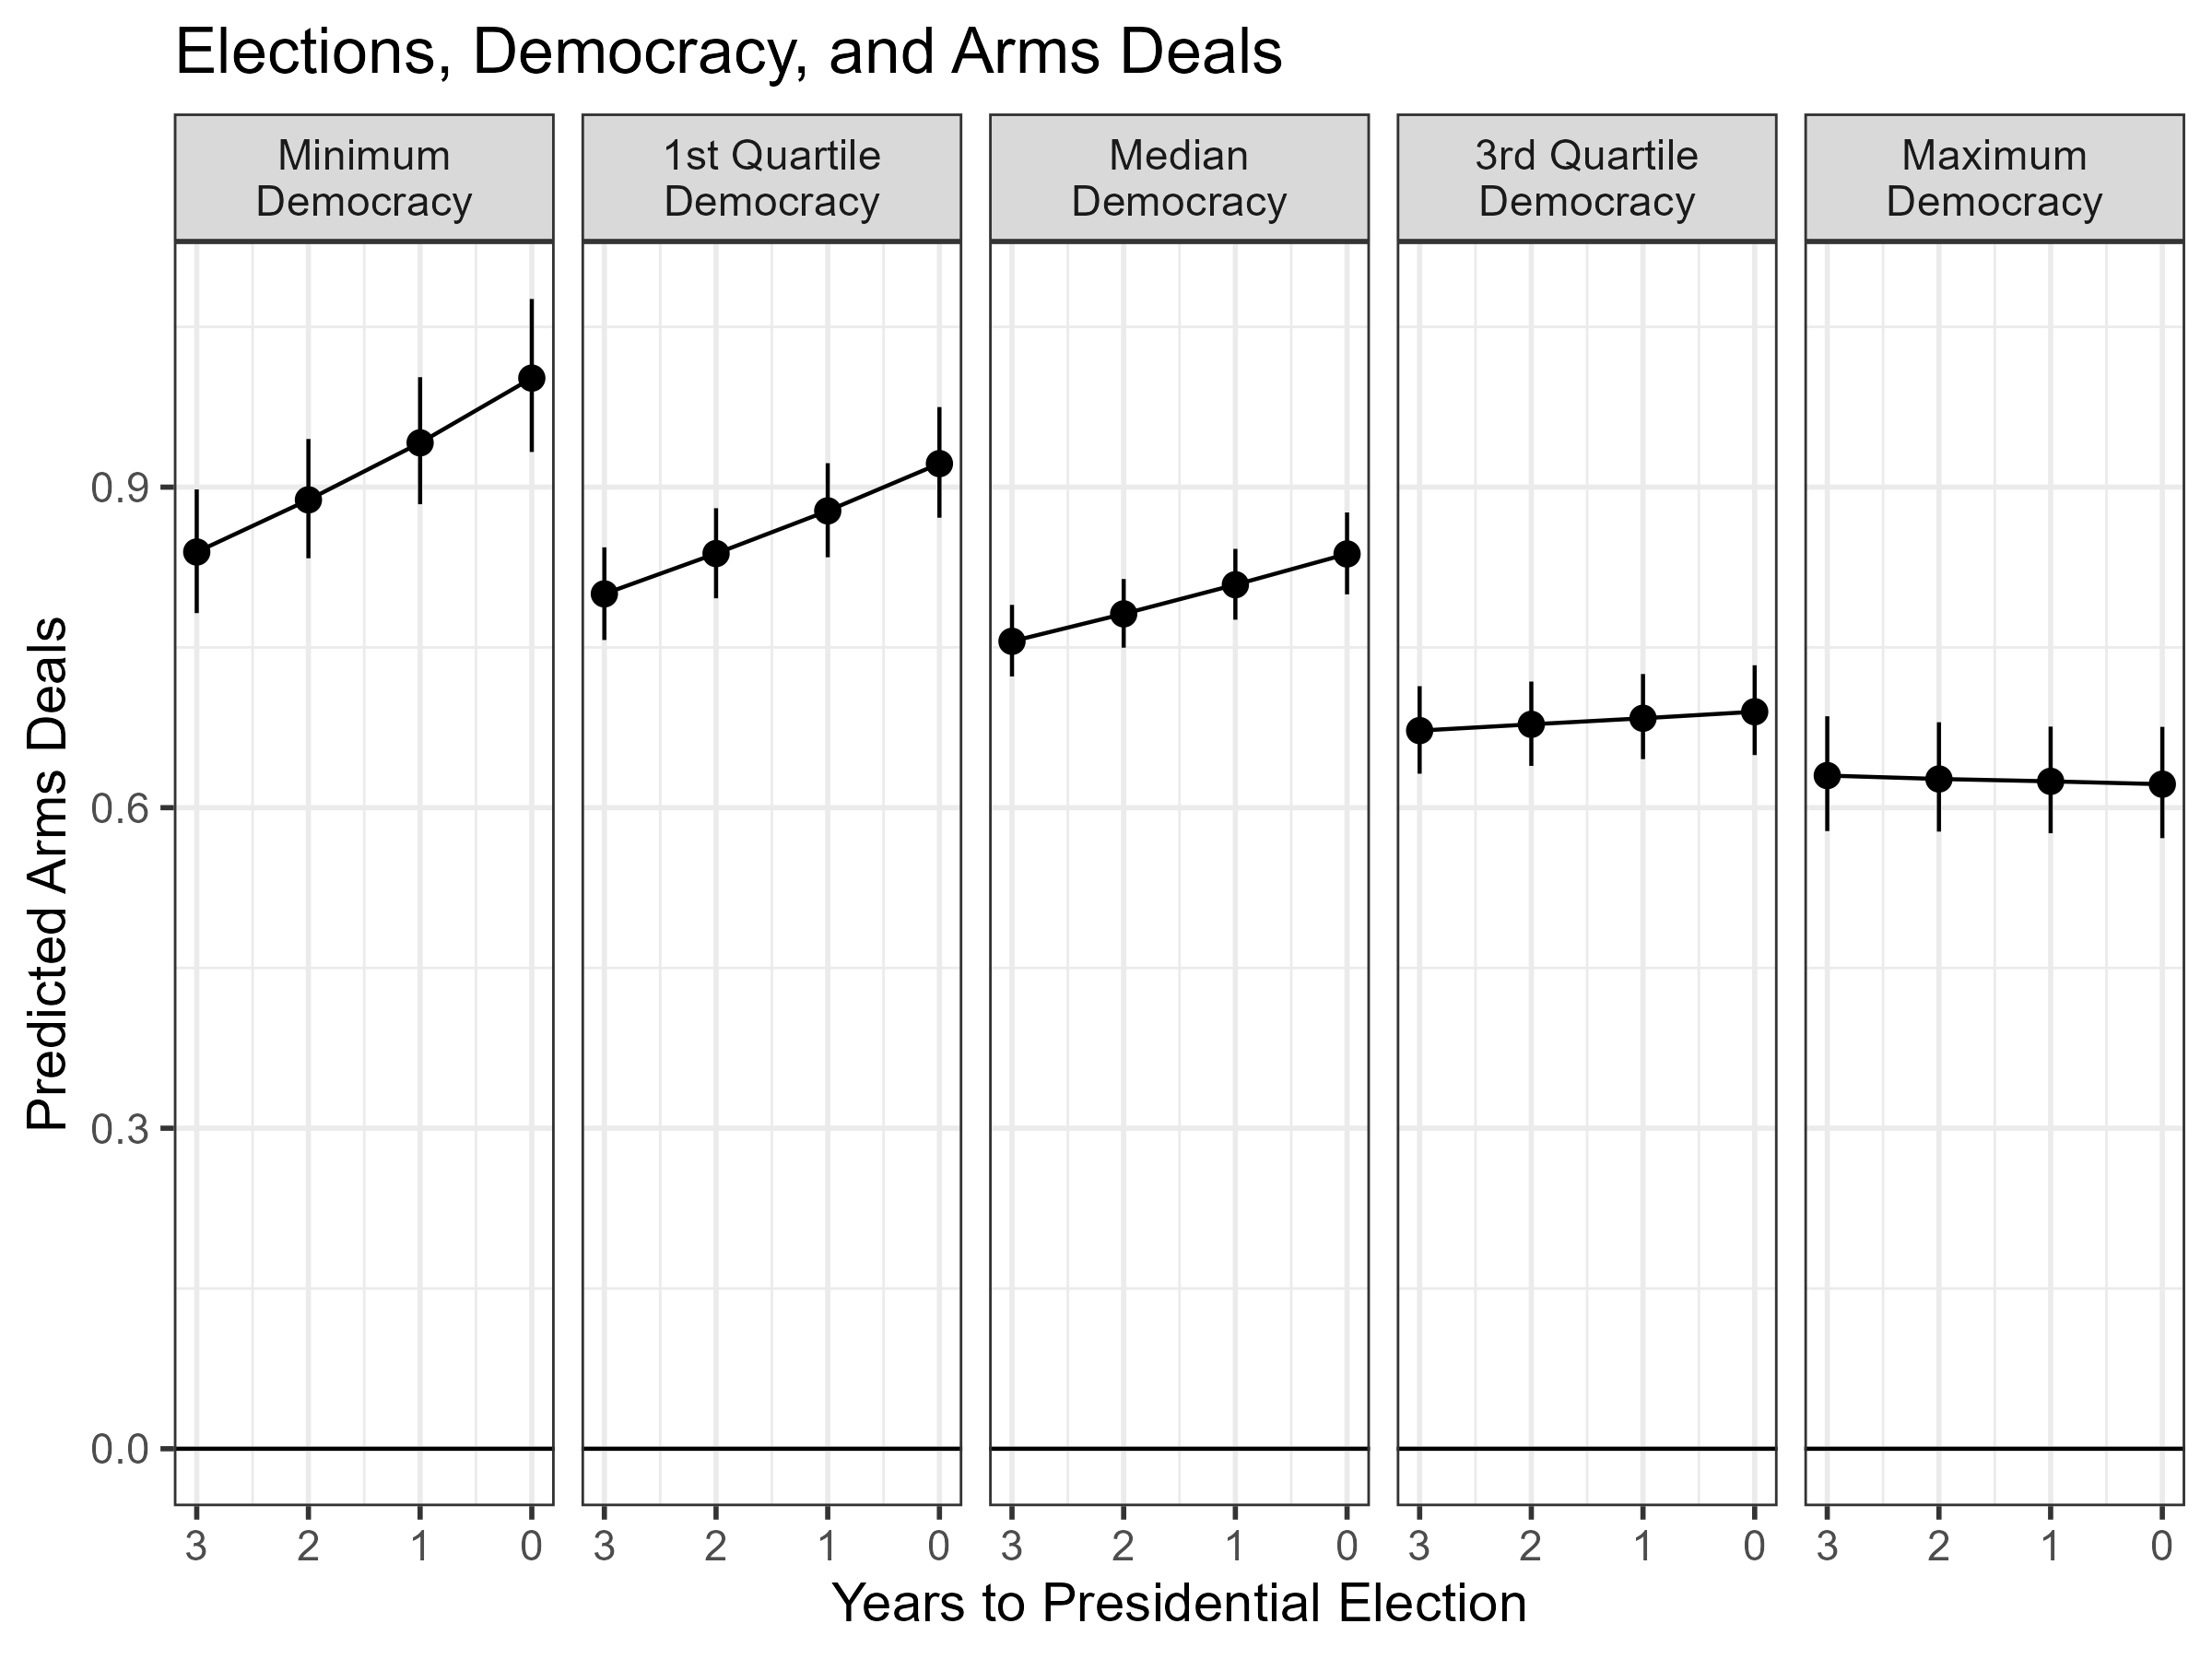
\includegraphics[width=0.95\textwidth]{../figures/democ-deals-pred.png}
	\caption{Predicted arms deals between the United States and five hypothetical states 1950 to 2014 based on presidential election proximity and partner democracy. Estimates derived from a hurdle Poisson model. Points mark the estimates and error bars summarize the 90\% credible interval.}
	\label{fig:democ-deals-pred}
\end{figure}


\autoref{fig:us-arms-plots} indicates that autocracies who clear the hurdle of buying any U.S. arms make more arms deals with the United States in election years.
During Congressional elections, which happen two years from presidential elections, arms deals rise slightly. 
Autocrats buy far more arms in presidential election years, as predicted deals for a hypothetical state with minimum polyarchy rise from 1.5 to 2.25. 
The entire posterior mass of the difference between one and zero years to an election is positive, with a 90\% credible interval from .46 to .68.
The arms deal increase in Congressional election years is half as large, with a 90\% credible interval between .13 and .34. 


Electoral increases when democracy is at the 1st quartile or median are smaller but clearly positive.
The arms deal cycle diminishes as democracy increases, so states with a polyarchy score above the third quartile see no change in arms deals during elections.
As a result, autocracies buy more arms during U.S. elections, especially presidential elections.


Whether autocracies make more or less arms deals than democracies depends on the presidential election cycle. 
Early in presidential terms, democracies make more arms deals. 
Democratic deals remain roughly constant across the electoral calendar because democracies engage in more peacetime defense cooperation. 
But in presidential election years, autocracies buy more U.S. arms. 
Thus, the political composition of U.S. arms deals depends on elections. 


In presidential and congressional election years, U.S. arms deals with autocracies rise.
My argument claims that U.S. leaders make these deals so they can award additional defense contracts to competitive electoral regions. 
If this is true, greater arms deals should increase defense contracting in swing states. 
The next analysis substantiates this claim.


\section{Arms Deals and Defense Contracting}


% describe the model 
Linking arms deals and defense contracting is challenging. 
Deals occur between countries, while defense contracting for electoral advantage takes place within U.S. states.
While jointly modeling deals with countries and contracts is theoretically possible, summing country-year deal estimates into an annual measure of total deals for the state-level analysis creates an aggregation problem. %\footnote{Separate time-series model of arms deals with autocracies and democracies over time could address this problem, but it would add enormous complexity.}
To maintain simplicity, this analysis uses observed annual deals, electoral competition and state-level factors to predict defense contract awards from 2001 to 2020. 
While connecting individual contracts and foreign military sales is challenging, the narrow focus on arms production and subsequent analysis examining deals cycles and contracts across defense industrial sectors mean that this approach still provides a useful test. 


I draw the outcome measure from Department of Defense prime contract award data in the USAspending.gov database.\footnote{Link here: \url{https://www.usaspending.gov/download_center/custom_award_data}.} 
This archive contains individual contracts from 2000 to 2020.
I analyze defense contracting in these years because archive starts in the 2000 fiscal year, detailed coverage begins in 2001 and some state-level controls have limited coverage after 2020.


Drawing on this contracting data trades temporal coverage for detailed information. 
Although other contracting datasets have more annual observations, they contain less information about state awards and what contracts cover. 
By using this data, I can examine the role of electoral geography, ensure that I am only capturing contracts for arms production and later link arms deals and contracts in defense industry sectors. 


The key outcome is total defense contracts for arms production awarded to each state every year, measured in millions of U.S. dollars.
This measure does not include sub-contracts, so it may not fully capture the location of funds. 
55\% of contracts require a subcontracting plan, so subcontracting is common but not uniform.  
While subcontracting is important, I analyze prime awards because these are more visible to leaders. 
I also focus on contracts for arms production, because arms deals should have little impact on contracts for other goods like construction equipment or food.
To do this, I filter the contracts using Department of Defense program description codes. 


Total defense contracts are challenging to model, because some states have zero and others have billions of arms contracting dollars. 
A zero-valued and right-skewed outcome results. 
Transforming such data can bias substantive effect calculations.
Traditional practices such as logging the outcome after adding one are sensitive to the outcome scale and what constant a researcher adds \citep{ChenRoth2022, MullahyNorton2022}. 


To overcome these issues, I fit two types of models.
First, I rescale the defense contracts measure to fall between zero and one by expressing each state's contracts as a share of total defense contracting in that year.
I then use ordered beta regression to model the rescaled outcome \citep{Kubinec2023}.\footnote{\url{https://www.robertkubinec.com/post/logs/}} 
Ordered beta regression fits bounded data better than other models with more restrictive distributional assumptions by using ordered cut points for boundary and continuous observations. 
This estimator employs a flexible outcome distribution and accounts for zeros.
It also avoids scale-effects from log-transformations and measuring contracts in millions of dollars. 
Converting the coefficients and marginal effects back to the outcome scale after estimation is straightforward, as I multiply the model estimates by the rescaling constant.


Because leveraging the flexibility and interpretability of ordered beta regression requires rescaling defense contracts, I present two additional checks in the appendix. 
First, I also fit a a hurdle lognormal model of contracts without any transformation.
Second, I model annual contract changes with a robust regression. 
Both alternatives give similar inferences.


The first independent variable is total annual arms deals.  
I measure arms deals by summing U.S. arms deals with all countries in every year. 
Annual deals range from 75 to 160. 


The other key independent variable is a dummy indicator of swing state status based on \citet{KrinerReeves2015}.
Swing states are states where the losing party won at least 45\% of the two-party vote in three straight elections.
These states are thus more competitive than others in the core Democratic or Republican coalitions, and could determine the outcome of an election.\footnote{In the appendix, I map the estimated consequences of a large increase in arms deals from 2007 to 2008.}
\autoref{tab:swing-list} lists the set of swing states and the years they are swing states.


\begin{table}[!h]

\caption{\label{tab:swing-list}: List of swing states.}
\centering
\fontsize{10}{12}\selectfont
\begin{tabular}[t]{lll}
\toprule
State & Start & End\\
\midrule
Arizona & 2017 & 2020\\
Colorado & 2009 & 2012\\
Florida & 2001 & 2020\\
Georgia & 2013 & 2020\\
Iowa & 2001 & 2012\\
Michigan & 2017 & 2020\\
Minnesota & 2005 & 2020\\
Missouri & 2005 & 2012\\
Nevada & 2001 & 2020\\
New Hampshire & 2001 & 2020\\
New Mexico & 2001 & 2008\\
North Carolina & 2005 & 2020\\
Ohio & 2001 & 2020\\
Pennsylvania & 2005 & 2020\\
Tennessee & 2000 & 2004\\
Virginia & 2001 & 2020\\
Wisconsin & 2001 & 2020\\
\bottomrule
\end{tabular}
\end{table}



I then interact the swing state dummy with total U.S. arms deals. 
The constituent term of arms deals, which expresses the association between deals and contracts outside of swing states, should be negligible or negative.
If leaders use arms deals for electoral advantage, then they will not be as correlated with contracts in less competitive areas. 
Because there are no years with zero U.S. arms deals, the swing state constituent term extrapolates far beyond the observed data, and is therefore not directly informative. 
The interaction of swing states and annual deals should be positive.


In addition to the electoral competition and deals variables, I include several controls. 
First, I adjust for population and GDP, because larger and more prosperous states receive more contracts. 
Other electoral competition indicators include the time to a presidential election and whether a state is a core member of the president's coalition \citep{KrinerReeves2015}. 
I also control for increased defense contracting demand during peak years in the global war on terror with a dummy variable that is equal to one from 2001 to 2011. 
The final control adjusts for presidential partisanship by dummy coding Republican presidencies. 


Further adjustments in the model account for the data structure.
I include state varying intercepts because observations cluster within states. 
Current contracting also depends on past contracting, but how much so varies across divergent state defense industries. 
I therefore add a state-specific lagged dependent variable, which allows temporal dependence in contracting to vary by state.\footnote{See the appendix for state parameter estimates.}


\subsection{Results}


To examine the arms deals and defense contracts hypothesis, I calculate the positive posterior mass of the interaction between arms deals and swing states. Because the hypothesis anticipates a positive association, posterior posterior mass gives corresponding evidence in the interaction term.\footnote{For the marginal effect of swing status and outcome predictions, I again use 90\% credible intervals.}
I then corroborate these estimates with marginal effects and predicted outcomes.


\autoref{fig:deals-swing-me} presents the interaction coefficient for deals and swing status, the marginal impact of swing state competition as arms deals vary, and predicted defense contracts for hypothetical swing and non-swing states. 
All these estimates suggest that deals increase defense contracting awards to swing states. 
In fact, swing states receive fewer contracts than other states in years with low arms deals. 


As the top left panel of \autoref{fig:deals-swing-me} shows, the impact of increasing arms deals on defense contracting is clearly positive in swing states and uncertain elsewhere.
98\% of the posterior mass of the deals and swing state interaction is positive, so the preponderance of evidence supports the deals and contracts hypothesis.
Only 34\% of the posterior mass in the deals constituent term is positive, however, so there is little evidence that deals increase contract awards outside of swing states. 


\begin{figure}[htpb]
	\centering
		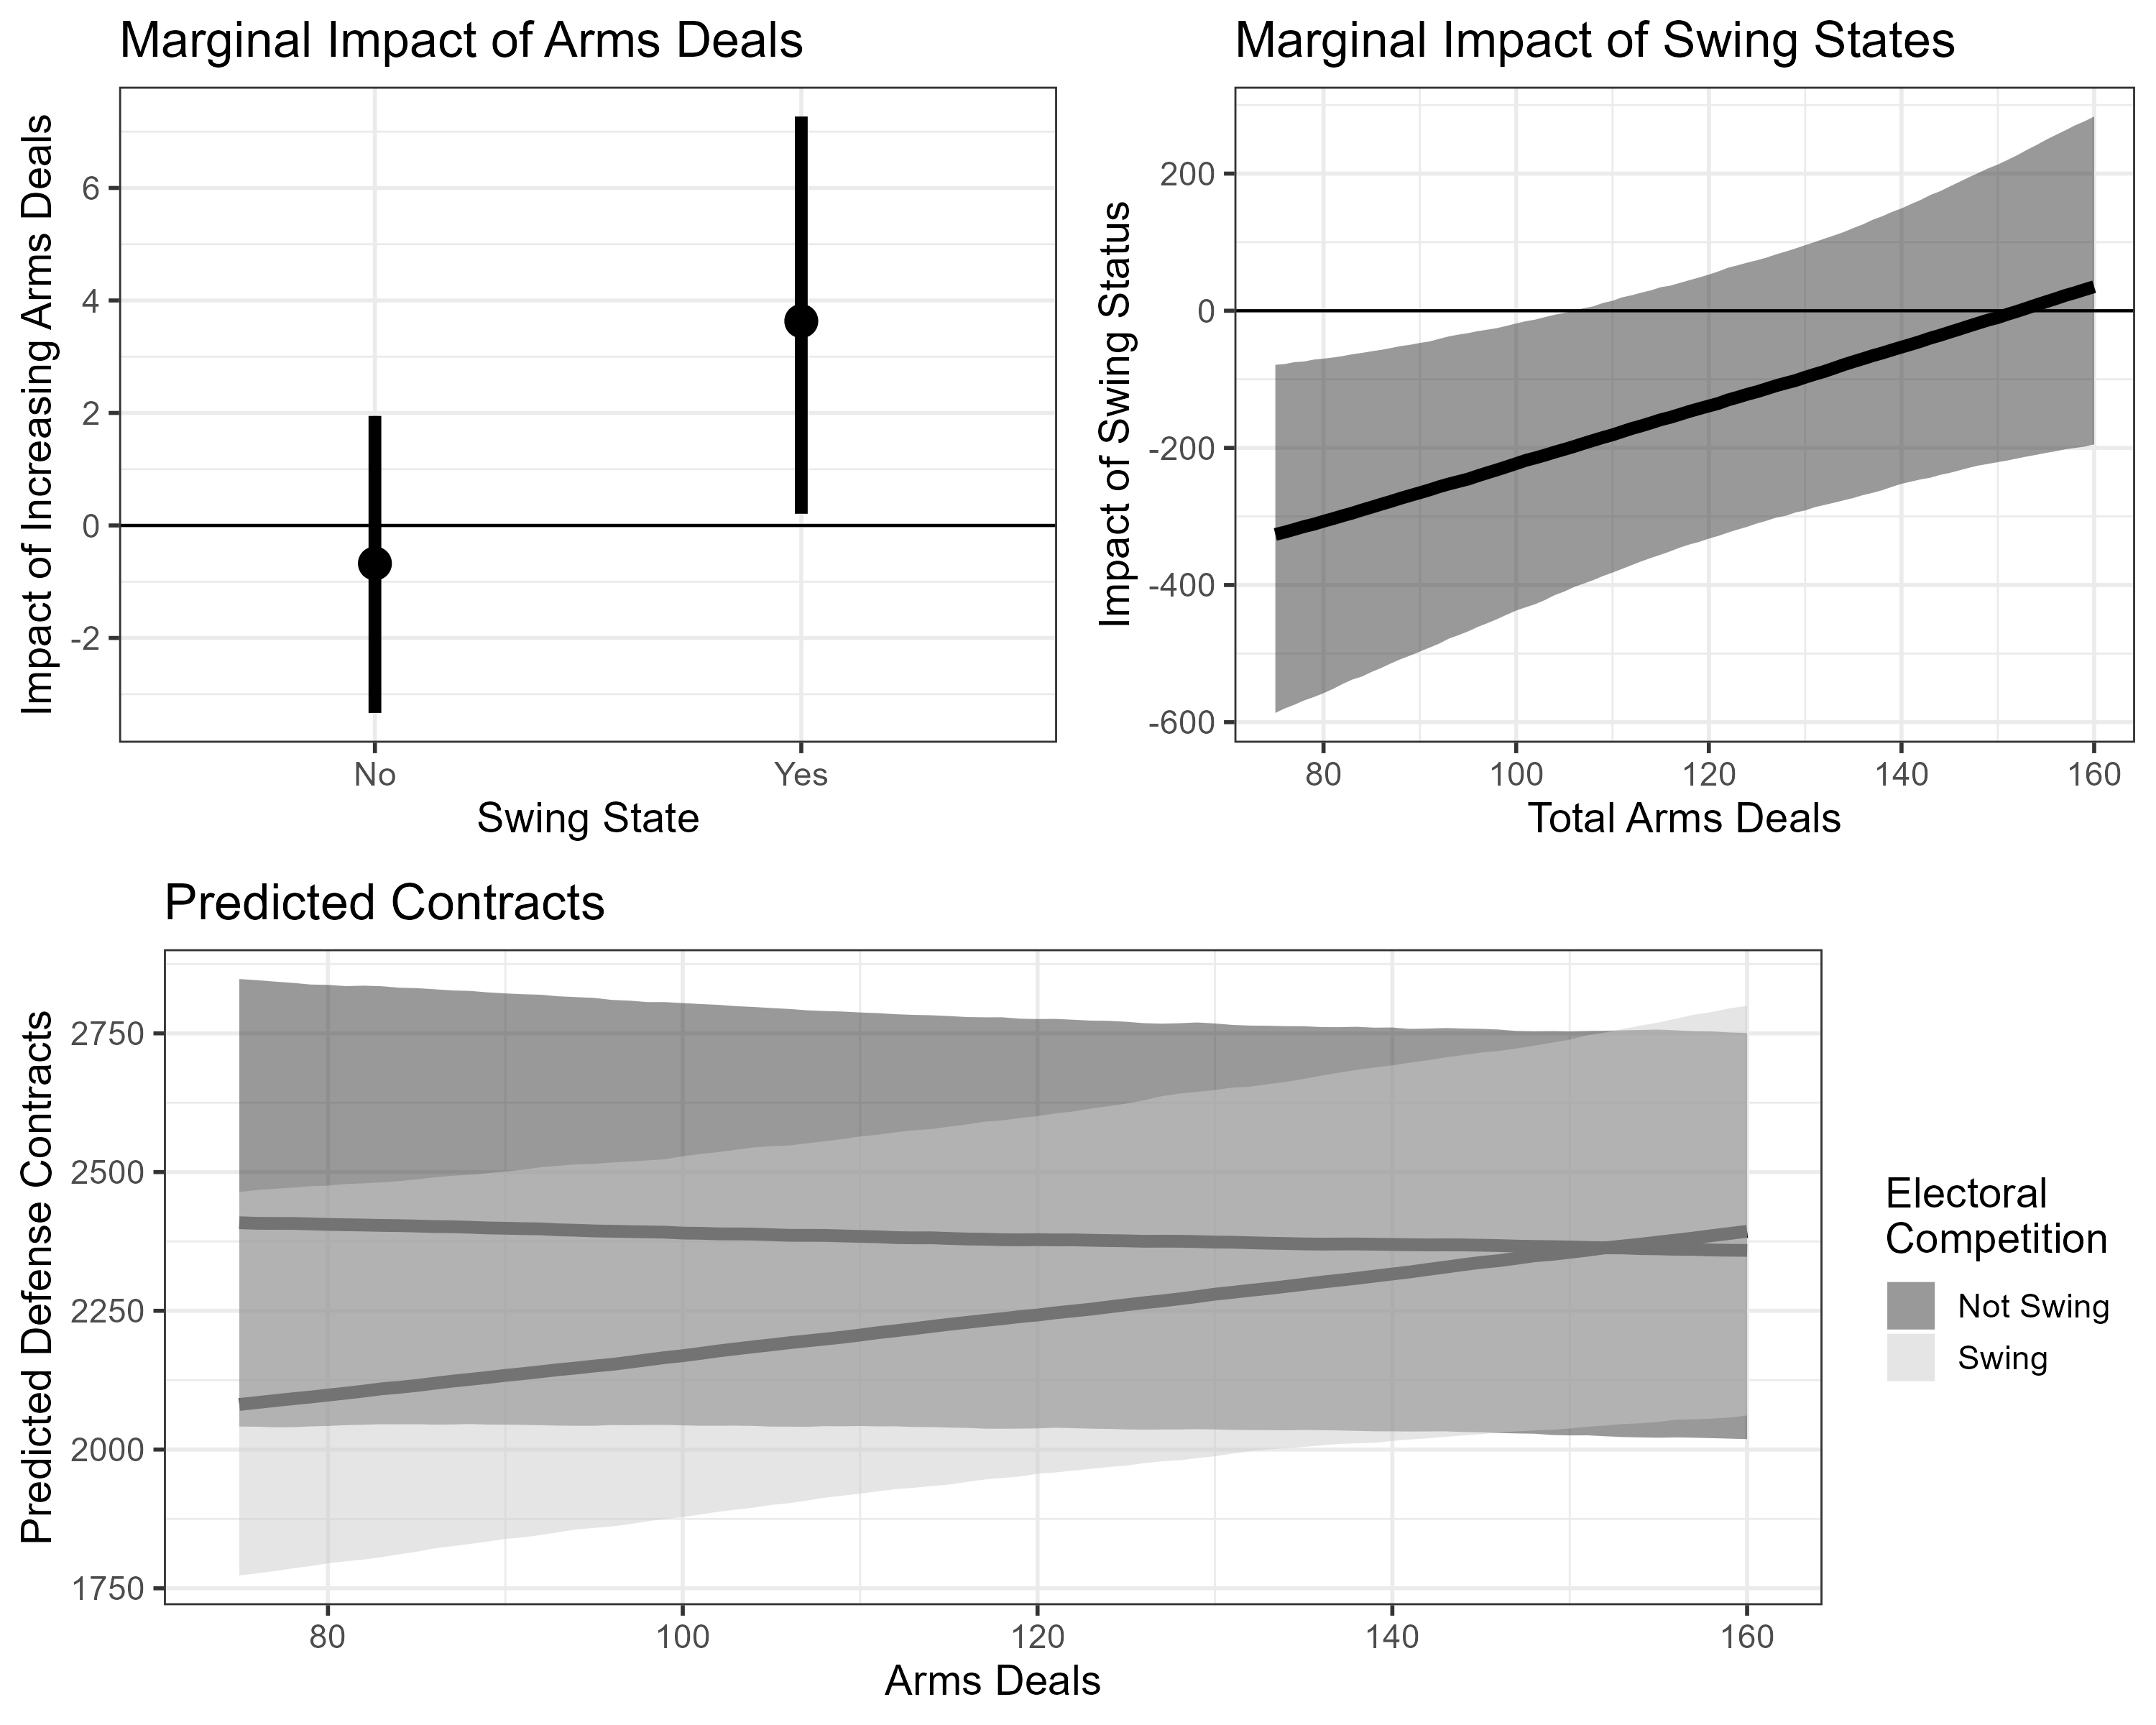
\includegraphics[width=0.95\textwidth]{../figures/deals-swing-me.png}
	\caption{Interaction coefficients, marginal effects and predicted outcomes from an interaction of swing state status and U.S. arms deals. The outcome is annual defense contracts in the 50 U.S. states from 2001 to 2020, measured in millions of dollars. Lines give the expected value, while the error bars summarize 90\% credible intervals. All other variables fixed at the mode or median. Estimates derived from an ordered beta regression with rescaled defense contracts, with estimates transformed back onto the outcome scale.}
	\label{fig:deals-swing-me}
\end{figure}


In addition to the direction of the relationship between deals and swing state contracts matching the argument, the correlation is substantively meaningful. 
Holding all else equal, moving from the first to the third quartile of deals increases defense contracting by \$202 million in a hypothetical swing state. 
This is a meaningful shift in defense contracting. 
Greater deals are less connected to contract awards outside swing states because the share of contracts that go to swing states rises in election years. 


The top right panel of \autoref{fig:deals-swing-me} shows that the marginal impact of swing state status on defense contracts rises as arms deals increase.  
Deals offset what is otherwise a swing state disadvantage in defense contracts. 
At the observed minimum of arms deals, a typical swing state receives \$300 million less in contract for arms production.
The swing state disadvantage at low levels of arms deals occurs because non-swing states like California and Texas have substantial defense industries.
When arms deals approach the observed maximum, swing states receive similar contracts to other states. 


Finally, predicted defense contracts increase as arms deals increase, but only in swing states, as I show in the bottom panel of \autoref{fig:deals-swing-me}. 
Holding all else equal, increasing arms deals leads to greater contracts in swing states. 
Defense contracts in non-swing states do not respond to increasing arms deals.
The gap in defense contracting between swing and other states thus disappears in years with high arms deals. 


All three of the quantities in  \autoref{fig:deals-swing-me} are consistent with one another and with the argument that leaders use arms deals to increase swing state contracts. 
Increasing arms deals are correlated with greater defense contracts in swing states. 
As a result, in years with more arms deals, swing states receive similar contracts to other states with larger economies and less electoral competition.


\section{Examining the Theoretical Process}


In this section, I unpack the process behind the argument.  
To begin, I check the argument that low constraint and additional security motivations drive autocracies to make arms deals.
After examining autocracies' rationale for making arms deals, I establish that the same platforms in arms deals between the United States and autocratic allies are also positively correlated with swing state contracts.
%If the platforms that moved in deals cycles were uncorrelated with swing state contracts, that would suggest any connection between deal cycles and swing state contracts is coincidental.
%The sectoral consistency I find instead suggests that arms deals do translate into swing state contracts.
Another process check in the appendix shows that the marginal impact of arms deals on swing state contracts is positive in the year before and year of a presidential election and is closer to zero otherwise.
This implies that leaders are more likely to channel contracts from arms deals to swing states around elections. 



\subsection{Why do Autocracies Make Arms Deals?}


% mechanisms
The argument claims that autocracies make arms deals with the United States near elections because their leaders have fewer constraints and reap security benefits. 
Here, I show that changes in political regime lead to changes in arms deal timing, which suggests that constraints matter. 
I then show that autocrats who are especially dependent on the United States for security, often make arms deals during elections.


\subsubsection{Low Constraint: Regime Changes}


To show how constraint changes deal timing, I compare arms deals in two U.S. allies under different political regimes. 
Greece and Portugal both underwent substantial regime changes, unlike other U.S. security partners that are consolidated democracies or autocracies. 
I selected these two states because the total variation in their polyarchy score is two times greater than average, they made arms deals with the United States across all regime types, they both democratized in the middle of the Cold War, and are both early members of NATO. 
Peacetime defense planning in NATO also makes these cases a hard test for the political constraint mechanism.


\begin{figure}[htpb]
	\centering
		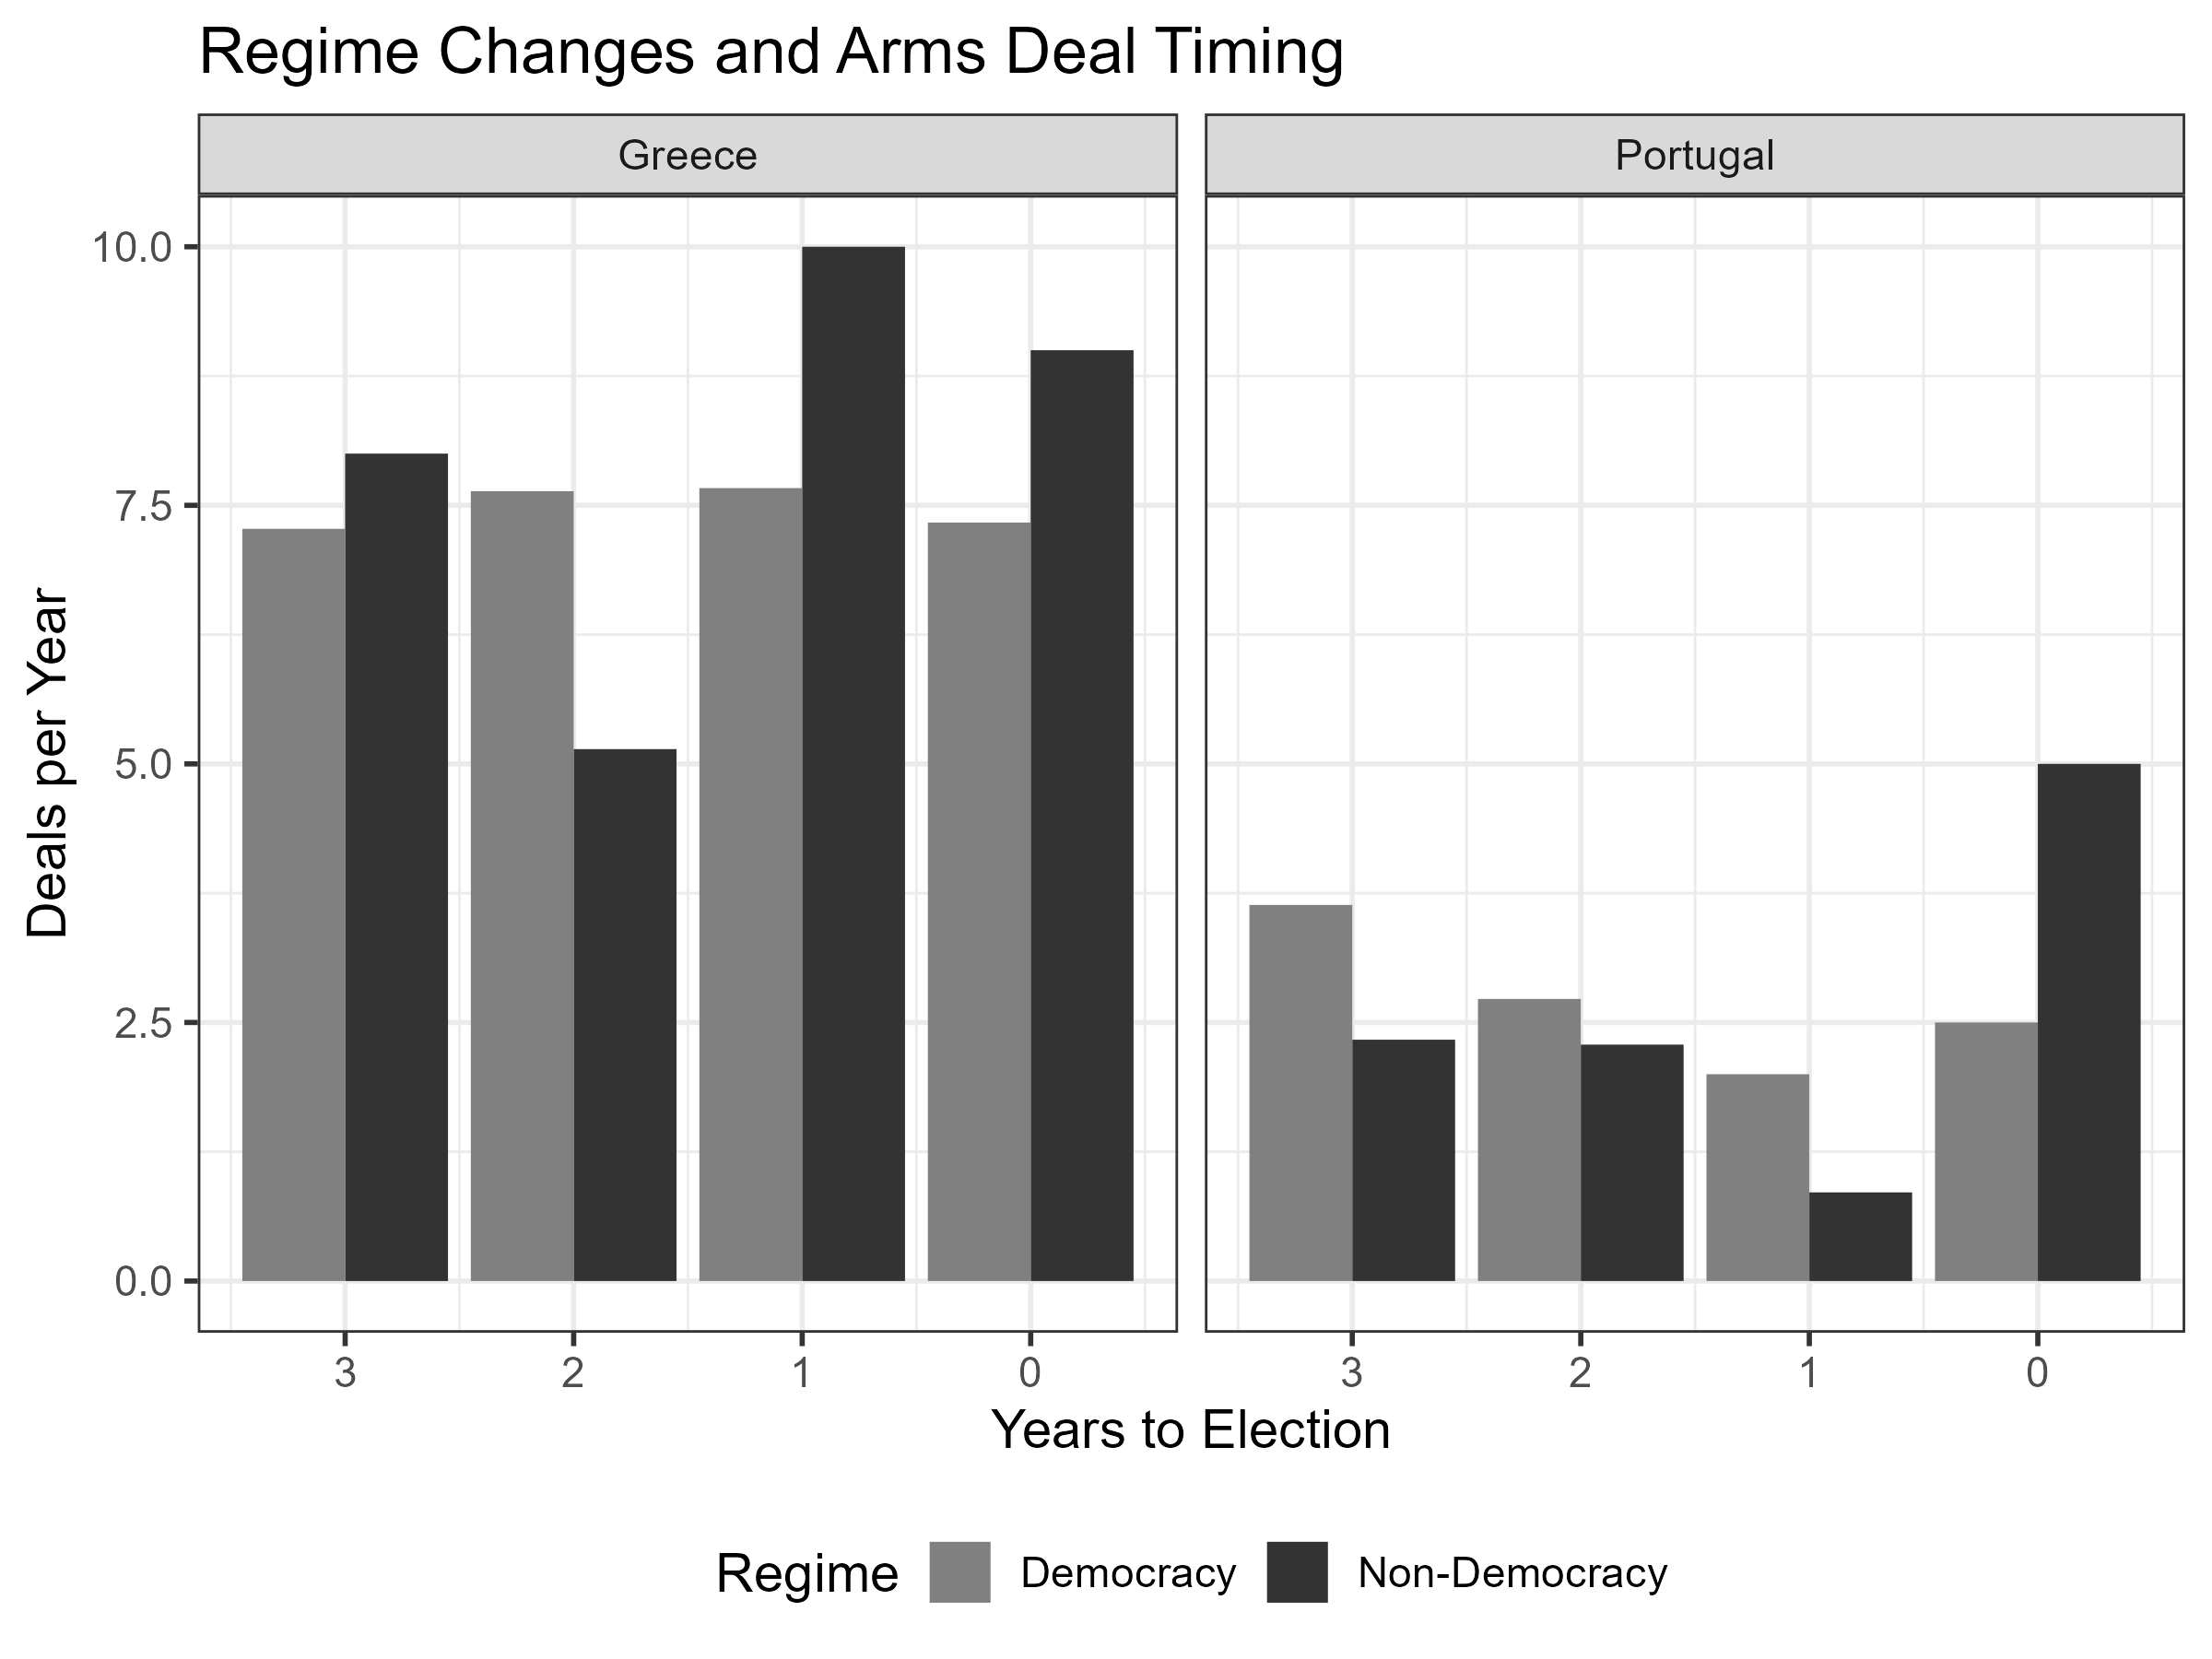
\includegraphics[width=0.95\textwidth]{../figures/deals-regime-change.png}
	\caption{Average U.S. arms deals with Greece and Portugal in every year of the presidential election cycle, divided by regime type. Democracy years have mean or greater polyarchy.}
	\label{fig:deals-regime-change}
\end{figure}


\autoref{fig:deals-regime-change} shows that for Greece and Portugal, autocratic periods are associated with buying more U.S. arms near presidential elections.
Conversely, arms deals are more stable in democratic years. 
On average, the Salazar regime in Portugal made 2.5 more arms deals in presidential election years than democratic Portuguese leaders.
During military rule, Greece made more arms deals in the year before and year of presidential elections.
After transitioning to democracy, Greece made consistent arms deals with the United States across the electoral cycle.


Even within NATO, autocratic leaders have more flexibility to make arms deals near presidential elections. 
Transitions to democracy attenuate this tendency, which suggests that democratic leaders face different constraints and incentives in when they acquire U.S. arms. 
Autocratic allies like the Salazar regime and Greek junta also have security reasons to make arms deals, which I detail below. 



\subsubsection{Security Motivation: Autocratic Allies}


I scrutinize autocrats' security motivation by examining U.S. allies. 
Because allies rely on the United States for security more than other autocracies, and U.S. leaders use arms to support autocratic partners \citep{Yarhi-Miloetal2016}, autocratic allies have additional motivation to purchase U.S. arms. 
Alliances consistently increase arms transfers \citep{Thurneretal2019}, and U.S. leaders can also more easily justify selling arms to perceived allies. 
As a result, allies should drive most of the increase in arms deals with autocracies near elections. 


%Alliances increase arms transfers in general. 
%\citet[pg. 184-5]{IkenberryGrieco2003} note that states often use direct transfers to attract and sustain security commitments. 


% security need
As I argued above, buying arms increases autocratic allies' security.
In addition to the capability boost of new arms, allies gain confidence in U.S. commitment because arms exports are a costly signal \citep{McManusYarhi-Milo2017}, and they win favor with U.S. leaders. 
Democratic allies gain security from closer peacetime defense cooperation and other commitment signals.


% less export cycles to non-allies
% each evidence sentence could be its own paragraph 
Furthermore, the security externalities of arms transfers reduce arms exports to non-allies. 
U.S. leaders will be less willing to increase the capability of states with fewer common interests, even if it facilitates contracting cycles.
Justifying deals with dictators is usually challenging, but it is more straightforward for perceived allies. 
U.S. allies that rely on American weapons, systems and doctrines can also integrate purchases more easily and build on past orders. 


% sum it up
%Among autocracies, U.S. allies have stronger security motivations because they depend on U.S. support and arms for security. 
%Alliances also make it easier for U.S. leaders to justify deals.
%As a result, 

Most of the electoral cycle in U.S. arms deals with autocracies should therefore occur with allied states. 
I tweak the hurdle Poisson model of autocracies and arms deals to examine this claim. 
To do this, I add the dummy indicator of whether a state is a U.S. ally to the interactions of partner regime and presidential election proximity.\footnote{The ally variable includes formal and informal allies.}
This creates triple interactions of alliance, regime type, and the election timing dummies. 


I summarize the interaction of alliances, democracy and presidential election proximity in \autoref{fig:us-arms-plots}.
This figure plots predicted arms deals based on proximity to a presidential election, democracy and alliance status. 
Each facet divides estimates based on democracy, while colors distinguish between allied and non-allied states. 


\begin{figure}[htpb]
	\centering
		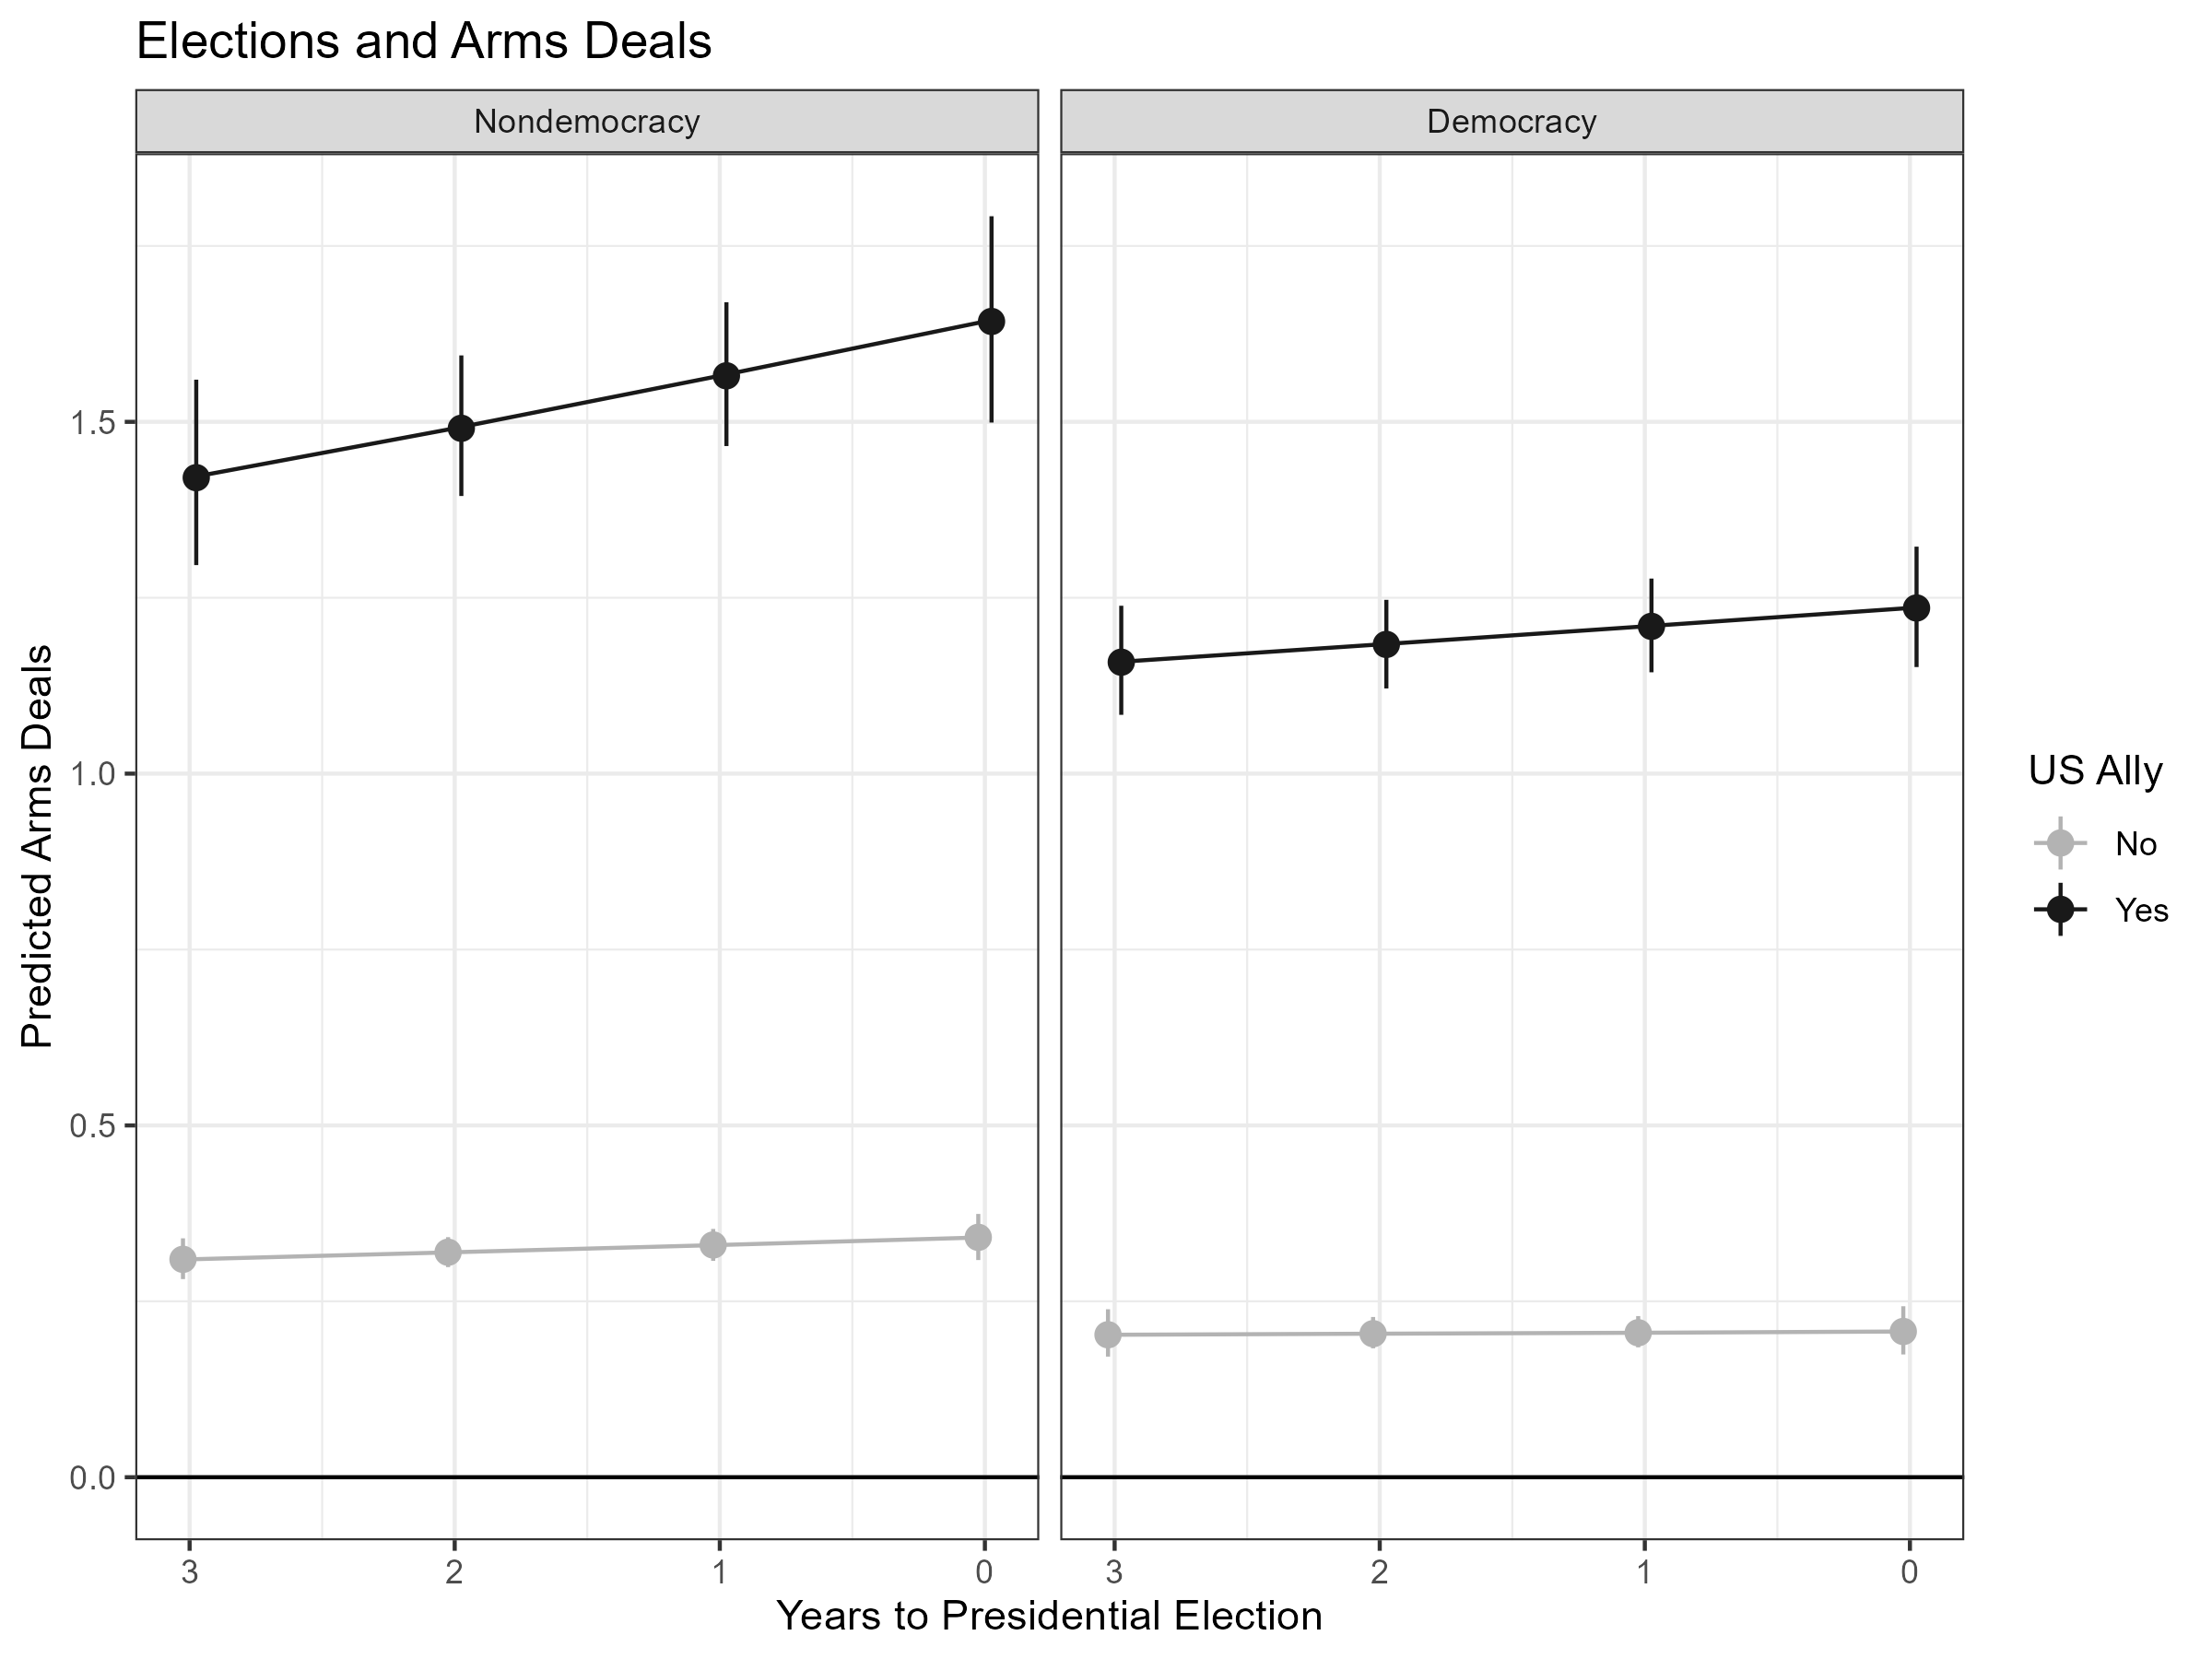
\includegraphics[width=0.95\textwidth]{../figures/us-arms-plots.png}
	\caption{Predicted arms deals between the United States and other states 1950 to 2014 based on presidential election proximity, democracy, and security alliances. Estimates derived from a hurdle Poisson model. Points mark the estimates and error bars summarize the 90\% credible interval. All other variables fixed to their mode or median.}
	\label{fig:us-arms-plots}
\end{figure}


The estimates in \autoref{fig:us-arms-plots} suggest that allies are responsible for most of the electoral cycle in U.S. arms deals with autocracies. 
The United States makes more arms deals with allied states than non-allied states, regardless of partner regime. 
Predicted deals with non-allied states are lower across all regimes. 


Autocratic allies are responsible for most purchases of U.S. arms in election years. 
When allied polyarchy is at the minimum, predicted arms deals rise from 2.2 to 2.9 in the year before and year of a presidential election. 
Congressional election years also see more deals between the United States and autocratic allies. 
Non-allied states with a minimal polyarchy score see predicted deals increase marginally in presidential election years.


Unlike autocratic allies, democratic allies receive consistent arms deals. 
These states have robust peacetime cooperation with the United States, and are more likely to benefit from other signals of commitment.
Alternative commitment signals, joint planning and constraints remove the means and motive for democracies to order more arms around presidential elections.


For autocratic allies of the United States, arms deals substitute for other security commitments, so they buy more U.S. arms. 
Autocracies with both political flexibility and security motivation buy arms around elections. 
In the next section, I use specific defense industrial sectors to check that connection between arms deals and defense contracts. 



\subsection{Which Weapons Drive Deals and Contracts?} 


The final process check examines whether the weapons systems that change hands in U.S. arms deals with autocratic allies are also correlated with swing-state contract awards. 
Showing that the United States makes more deals for specific weapons around elections, and that deals for those weapons correlate with defense contract awards in swing states increases confidence in the theoretical process.\footnote{These correlations do not link specific deals and contracts, however.}
I find that the electoral rise in U.S. arms deals with autocracies includes deals for aircraft, ships and vehicles, all of which also increase swing state contracts. 
These three systems have widely distributed production bases and comprise 69\% of all deals. 
Aircraft deals are especially likely to increase swing state contracts, given dispersed supply chains and high value. 


To analyze weapon types, I divided arms deals and defense contracts into six matching sectors. 
These include aircraft, arms and munitions, military electronics, missiles and space technology, ships, and vehicles.  
Each sector has a distinct production geography and arms deal distribution.


I then fit six hurdle Poisson models of arms deals, one for each type of arms. 
This outcome is deals in each sector for every country-year observation. 
These models use the same predictors as the main arms deals model; the interaction of recipient democracy and election timing, along with a hurdle equation and controls.
Using the hurdle further improves model fit because more country-year observations have zero deals within sectors. 


For ease of presentation, I plot predicted arms deals at the minimum and maximum of partner democracy in \autoref{fig:deals-sector}.
The estimates suggest that a combination of weapons systems drive electoral cycles in arms deals with autocratic allies.  


Aircraft deals are the most common overall with 48\% of all deals, and autocracies buy more aircraft in election years.
In expectation, aircraft deals with autocrats rise by .4 in presidential election years, albeit from a lower base in the preceding year.\footnote{The difference between 3 years to an election and an election year has a 90\% credible interval from 0.09 to 0.26.}
Aircraft deals with democratic allies respond less to elections, perhaps because autocrats weaker domestic production of aircraft. 


\begin{figure}[htpb]
	\centering
		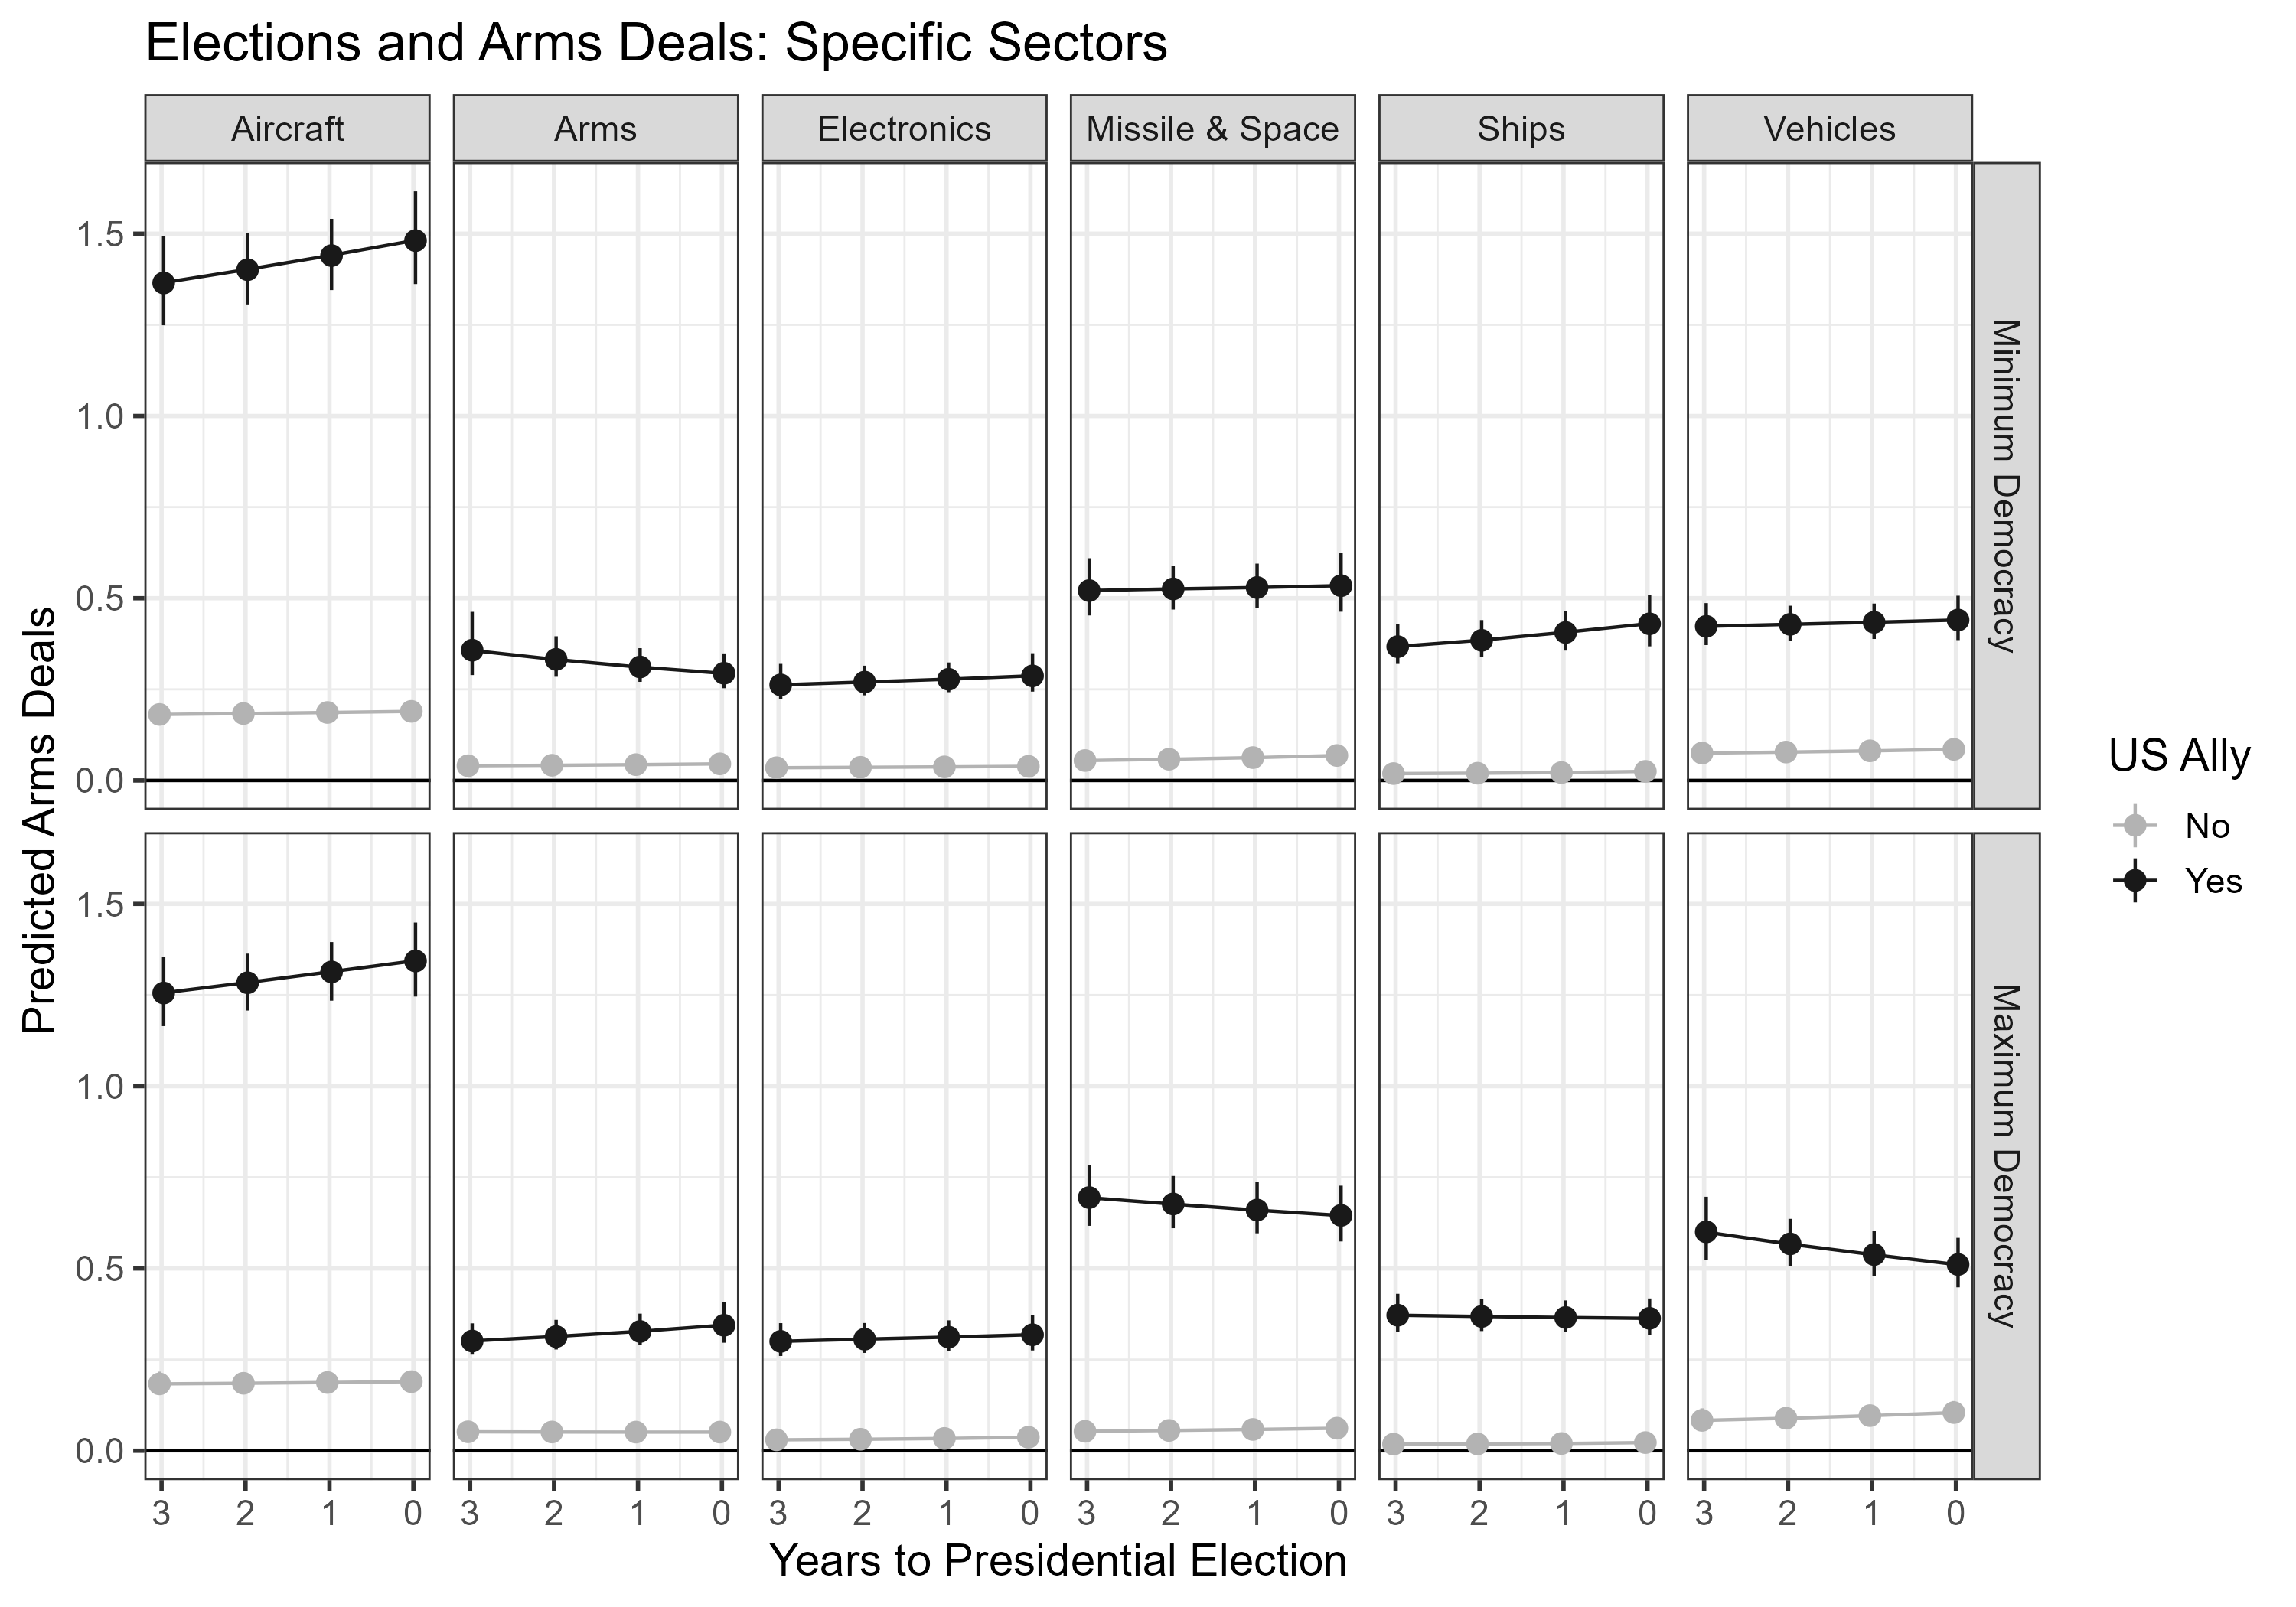
\includegraphics[width=0.95\textwidth]{../figures/deals-sector.png}
	\caption{Predicted arms deals between the United States and other states 1950 to 2020 based on presidential election proximity, democracy, and military alliance. Estimates derived from six sector-specific hurdle Poisson models counting annual deals divided by the type of military good exchanged. Points mark the estimates and error bars summarize the 90\% credible interval. All other variables fixed to their mode or median.}
	\label{fig:deals-sector}
\end{figure}


Among autocracies, arms, ships and vehicle deals also increase in election years, though far less than aircraft. 
Perhaps due to weaker domestic production, autocracies buy more electronics than democracies. 
Deals for arms and ships increase in presidential election years, and democracies strike more deals for both.  
Democratic deals for these weapons do not track elections in the same way, although democracies buy more ships in Congressional election years. 


Other weapons show less evidence of autocratic cycles in arms deals. 
Democratic allies are more likely to make deals for missiles and space systems, and deal timing is similar across regimes. 
The importance of democracy for missile technology likely reflects joint production and planning in formal U.S. alliances. 


Aircraft, munitions, ships and vehicles all change hands in autocratic deal cycles. 
Deals for these weapons are also positively correlated with swing state contracts.  



\subsubsection{Deals and Defense Contracts by Sector}


I fit six models of defense contracts to examine the deals and contracts hypothesis for each sector and check if the sectors with deal cycles have a positive association between deals and swing state contracts. 
This analysis divides total contracts by sector using the product description for each contract. 
As in the analysis of aggregate defense contracting, I rescale the outcome between 0 and 1 using the annual sum of contracts for those sectors. 
I then fit ordered beta regression models of the rescaled outcomes, using an identical specification to the aggregate defense contracting model.
The key independent variables in these models are observed arms deals in each sector, the binary swing state indicator, and their interaction. 
I also include the same set of state varying intercepts, state-specific autocorrelation, and other controls. 


\autoref{fig:me-deals-sector} plots the interaction between six types of arms deals and swing state status.  
These estimates show the deals coefficients from six ordered beta models, transformed back to the outcome scale. 
Again, I focus on the positive posterior mass, as this gives the evidence consistent with the directional deals and contracts hypothesis.


\begin{figure}[htpb]
	\centering
		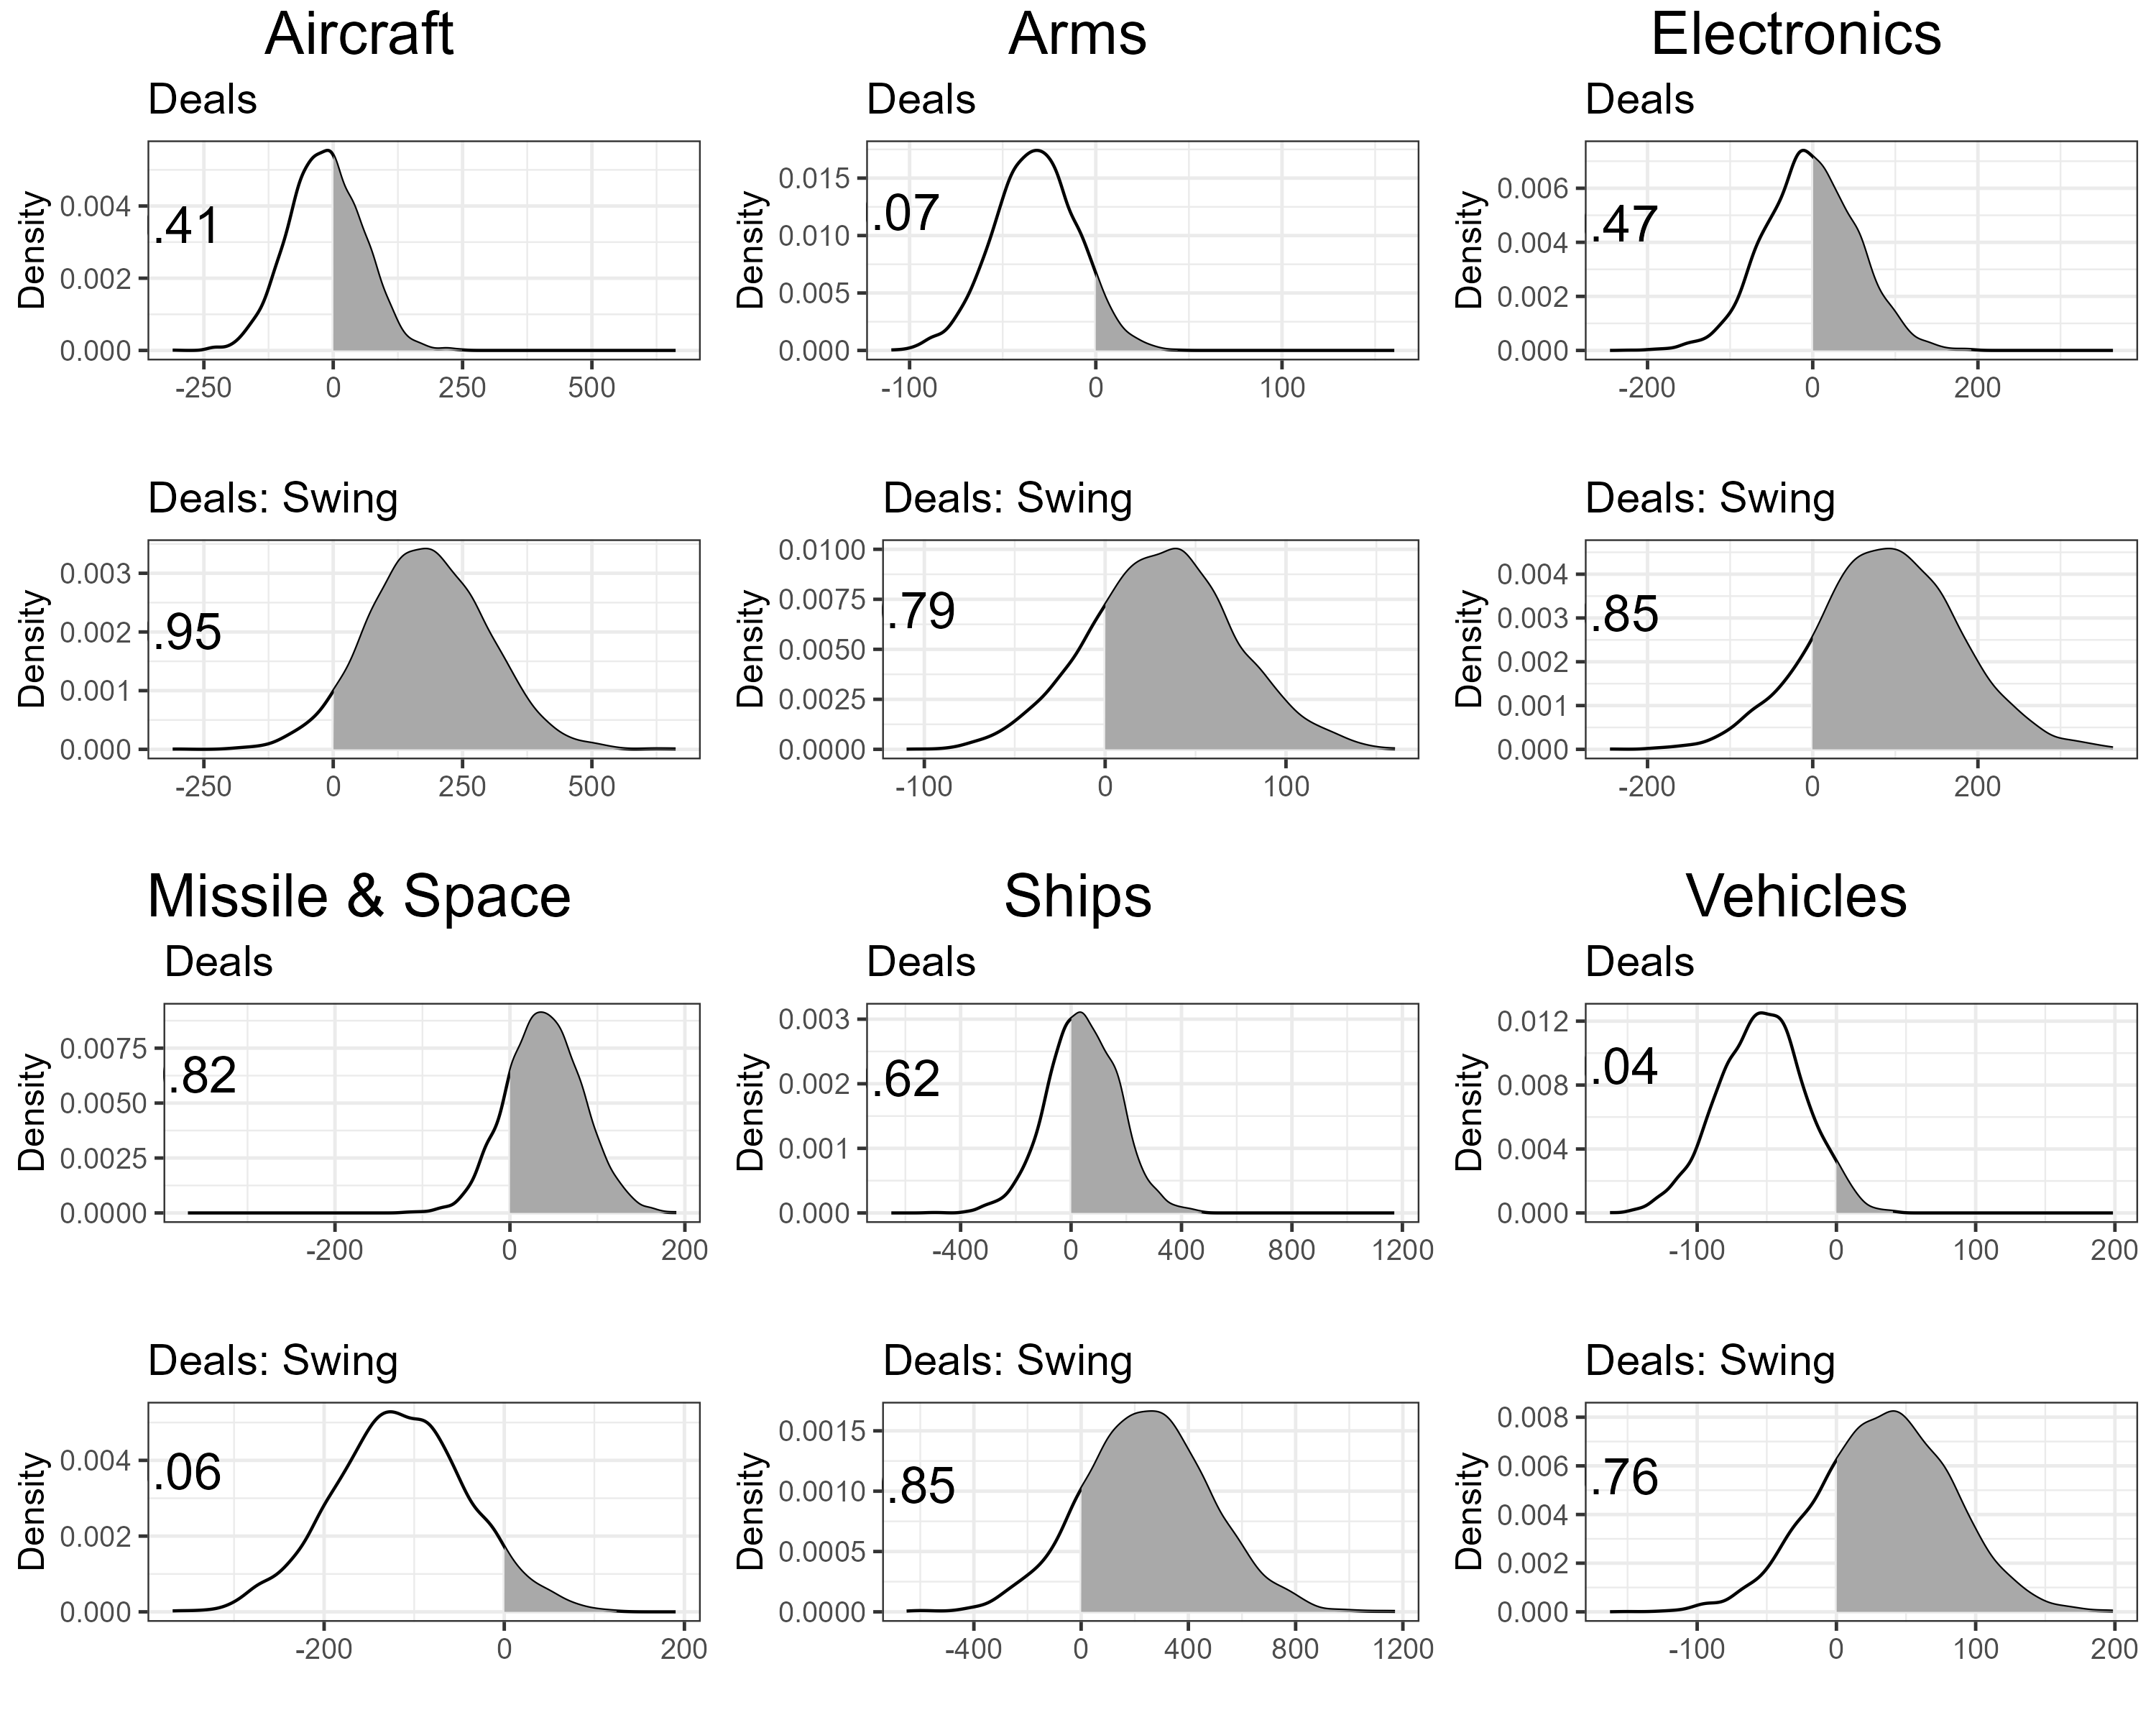
\includegraphics[width=0.95\textwidth]{../figures/me-deals-sector.png}
	\caption{Associations between different types of arms deals and defense contracts within defense industry sectors. Shaded area and text summarize the positive posterior mass. Estimates in millions of U.S. dollars.}
	\label{fig:me-deals-sector}
\end{figure}


While deals for arms, vehicles, and missile and space components have largely positive associations with corresponding swing state contracts, aircraft deals have the greatest positive relationship. 
95\% of the posterior mass in the interaction of aircraft deals and swing state status is positive.
This reflects a diffuse supply chain for engines, airframes, and other components as well as the value of aircraft.


In addition to aircraft, ships and electronic deals are correlated with greater swing state contracts. 
An additional ship deal is associated with \$300 million more contracts in a hypothetical swing state. 
Total annual ships deals range from one to 11, so these deals are rare but lucrative. 
The impact also may not concentrate in coastal state shipyards, as most ships deals move whole platforms, which require components from elsewhere. 


Similarly, much of the vehicles posterior mass is positive in swing states, though the direction of that association is less clear.
Most of the correlation between electronics deals and swing state contracts for military electronics is positive as well.
As a result, the main platforms that move in deals near elections also increase swing state contracts. 


Only missile and space production, which is geographically concentrated, has greater positive mass on the association between deals and contracts outside of swing states. 
Perhaps as a result, the United States does not sell many more missile and space systems to autocracies near presidential elections. 
Munitions have a positive association with swing state contracts, but there is little evidence of cyclical deals in this sector. 


Autocratic purchases of aircraft, arms, ships and vehicles drive increasing swing state contracts.
Aircraft and ship deals are particularly lucrative for swing state contracts. 



\section{Discussion and Conclusion}


Electoral competition in the United States encourages arms transfers to autocracies like the Shah of Iran, Latin American juntas and Saudi Arabia.
To improve or maintain economic conditions, leaders strike additional arms deals with autocracies in election years.
Deals increase swing state contract awards and allow leaders to claim credit for protecting or adding jobs.
For their part, autocracies take arms because they gain security and have greater political flexibility in when they buy arms. 


The argument and results link scholarship on security cooperation and political budget cycles. 
Security cooperation with arms sales helps leaders award contracts with less attention to the budget process and force planning of the U.S. military.
This mirrors how states manipulate international economic ties to undermine adversarial leaders \citep{KimMargalit2021}.


% alliance value and autoc alliance durability
Along with adding an electoral rationale for U.S. arms sales, this paper helps explain why U.S. security cooperation with autocracies endures despite normative and practical criticisms. 
Arms deals increase autocracies security and help U.S. leaders win elections.
These informal linkages are essential to grand bargains between the United States and its security prot{\'e}g{\'e}s.
%Electoral arms deals sustain regular cooperation across regimes.
%Allies need not undertake these cycles deliberately, but making arms deals is part of a cooperative bundle of ties.


% limitations 
There are some limitations to the argument and findings.
First, I focus on the United States as a most-likely case of elections stimulating arms deals. 
Other democracies may use autocratic arms deals to support employment, but the process will differ. 
Second, the results do not present a unified model of deals and contracts, and do not link specific deals and contracts. 


Future research could proceed in several directions. 
Exploring the role of defense industry integration and intermediate goods in electoral arms deal cycles is interesting.
Scholars might also examine other democratic arms exporters and consider other ways that leaders leverage security cooperation to try and win elections. 


Electoral competition reshapes international security cooperation.
Using defense contracting to improve the economy during elections encourages U.S. arms deals with autocracies.
While these deals may send U.S. arms to risky destinations, electoral considerations win out. 


\newpage
\singlespace
 
\bibliography{../../MasterBibliography} 


\end{document}
